\documentclass[10pt,pdf,hyperref={unicode}]{beamer}

\usetheme[progressbar=frametitle]{metropolis}
\usepackage{booktabs}
\usepackage[scale=2]{ccicons}
\usepackage{pgfplots}
\usepgfplotslibrary{dateplot}
\usepackage{xspace}
\newcommand{\themename}{\textbf{\textsc{metropolis}}\xspace}
\usepackage{multicol}
\usepackage[T2A]{fontenc}
\usepackage[utf8]{inputenc}
\usepackage{listings}
\usepackage{hyperref}
\usepackage{textcomp}


\usetheme{Pittsburgh}
\usecolortheme{seahorse}
\definecolor{light-gray}{gray}{0.90}


\lstset{
  language=C++,                % choose the language of the code
  basicstyle=\linespread{1.1}\ttfamily,
  columns=fixed,
  fontadjust=true,
  basewidth=0.5em,
  keywordstyle=\color{blue}\bfseries,
  commentstyle=\color{gray},
  stringstyle=\ttfamily\color{orange!50!black},
  showstringspaces=false,
  numbersep=5pt,
  numberstyle=\tiny\color{black},
  numberfirstline=true,
  stepnumber=1,                   % the step between two line-numbers.        
  numbersep=10pt,                  % how far the line-numbers are from the code
  backgroundcolor=\color{black!2},  % choose the background color. You must add \usepackage{color}
  showstringspaces=false,         % underline spaces within strings
  captionpos=b,                   % sets the caption-position to bottom
  breaklines=true,                % sets automatic line breaking
  breakatwhitespace=true,         % sets if automatic breaks should only happen at whitespace
  xleftmargin=.2in,
  extendedchars=\true,
  keepspaces = true,
}

\newcommand\upquote[1]{\textquotesingle#1\textquotesingle}


\title{Работа с изображениями в языке C++}
\author{Бирюков В. А.} 
\date{\today}
\begin{document}

\begin{frame}
\titlepage
\end{frame} 


\begin{frame}[fragile]
\frametitle{Шестнадцатеричная система} 
Система счисления по целочисленному основанию \texttt{16}. \\ 
В качестве цифр этой системы обычно используются цифры от \texttt{0} до \texttt{9} и латинские буквы от \texttt{A} до \texttt{F}.\\
Примеры:\\
\begin{multicols}{2}
\texttt{6 =  0x6} \\
\texttt{12 = 0xc} \\
\texttt{20 = 0x14} \\
\texttt{200 = 0xc8} \\
\texttt{255 = 0xff} \\
\texttt{256 = 0x100} \\
\texttt{1000 = 0x3E8} \\
\texttt{1024 = 0x400} \\
\end{multicols}
\end{frame}


\begin{frame}[fragile]
\frametitle{Коды ASCII в шестнадцатеричной системе} 
Коды ASCII в шестнадцатеричной системе:\\
\begin{multicols}{4}
\texttt{\upquote{\textbackslash 0} =  0x00} \\
\texttt{\upquote{\textbackslash n} =  0x0a} \\
\texttt{\upquote{\textbackslash r} = 0x0d} \\
\texttt{\upquote{ } = 0x20} \\
\texttt{\upquote{0} = 0x30} \\
\texttt{\upquote{1} = 0x31} \\
\texttt{\upquote{2} = 0x32} \\
\texttt{\upquote{3} = 0x33} \\
\texttt{\upquote{A} = 0x41} \\
\texttt{\upquote{B} = 0x42} \\
\texttt{\upquote{P} = 0x50} \\
\texttt{\upquote{Z} = 0x5A} \\
\texttt{\upquote{a} = 0x61} \\
\texttt{\upquote{b} = 0x62} \\
\texttt{\upquote{p} = 0x70} \\
\texttt{\upquote{z} = 0x7a} \\
\end{multicols}
\end{frame}


\begin{frame}[fragile]
\frametitle{Сохраняем строку в файл}
Текстовый режим открытия файла:
\begin{lstlisting}
std::ofstream out{"my_file.txt"};
out << "Cat\nDog";
\end{lstlisting}
То в файл запишется (Linux):\\
\noindent\fbox{
\parbox{0.5\textwidth}{
\texttt{%
43 61 74 0a 44 6f 67
}
}
}\\
Или в файл запишется (Windows):\\
\noindent\fbox{
\parbox{0.5\textwidth}{
\texttt{%
43 61 74 0d 0a 44 6f 67
}
}
}
\end{frame}


\begin{frame}[fragile]
\frametitle{Сохраняем строку в файл}
Бинарный режим открытия файла:
\begin{lstlisting}
std::ofstream out{"my_file.txt", std::ios::binary};
out << "Cat\nDog";
\end{lstlisting}

То в файл запишется (Linux и Windows):\\
\noindent\fbox{
\parbox{0.5\textwidth}{
\texttt{%
43 61 74 0a 44 6f 67
}
}
}
\end{frame}

\begin{frame}[fragile]
\frametitle{Сохраняем число в файл}
\begin{lstlisting}
int a = 12345678;
std::ofstream out{"my_file.txt"};
out << a;
\end{lstlisting}
То в файл запишется строка, представляющая число 12345678:\\
\noindent\fbox{
\parbox{0.5\textwidth}{
\texttt{%
31 32 33 34 35 36 37 38
}
}
}\\
\end{frame}

\begin{frame}[fragile]
\frametitle{Сохраняем число в файл}
\begin{lstlisting}
int a = 12345678; // 12345678 == 0xBC614E
std::ofstream out{"my_file.txt", std::ios::binary};
out.write(reinterpret_cast<const char*>(&a), 4);
\end{lstlisting}
То в файл запишется байтовое представления числа в памяти:\\
\noindent\fbox{
\parbox{0.5\textwidth}{
\texttt{%
4E 61 BC 00
}
}
}\\
\end{frame}

\begin{frame}[fragile]
\frametitle{Сохраняем \texttt{unsigned char} в файл}
Числа типа \texttt{unsigned char} и \texttt{char} воспринимаются оператором \texttt{<{}<} как символы.
\begin{lstlisting}
unsigned char a = 75; // 75 = 0x4b
std::ofstream out{"my_file.txt"};
out << a;
\end{lstlisting}
То в файл запишется символ \texttt{K}:\\
\noindent\fbox{\parbox{0.5\textwidth}{\texttt{4B}}}\\
Если вы откроете этот файл в текстовом редакторе, то увидите:
\noindent\fbox{\parbox{0.5\textwidth}{\texttt{K}}}\\
\end{frame}


\begin{frame}[fragile]
\frametitle{Сохраняем \texttt{unsigned char} в файл}
Чтобы число типа \texttt{unsigned char} воспринимается оператором \texttt{<{}<} как число,
нужно привести его к другому целочисленному типу.
\begin{lstlisting}
unsigned char a = 75; // 75 = 0x4b
std::ofstream out{"my_file.txt"};
out << static_cast<int>(a);
\end{lstlisting}
То в файл запишется символ \texttt{K}:\\
\noindent\fbox{\parbox{0.5\textwidth}{\texttt{37 35}}}\\
Если вы откроете этот файл в текстовом редакторе, то увидите:
\noindent\fbox{\parbox{0.5\textwidth}{\texttt{75}}}\\
\end{frame}


\begin{frame}[fragile]
\frametitle{Сохраняем \texttt{unsigned char} в файл}
Числа типа \texttt{unsigned char} и \texttt{char} воспринимаются оператором \texttt{<{}<} как символы.
\begin{lstlisting}
unsigned char a = 75; // 75 = 0x4b
std::ofstream out{"my_file.txt", std::ios::binary};
out.write(reinterpret_cast<const char*>(&a), 1);
\end{lstlisting}
То в файл запишется байтовое представление числа:\\
\noindent\fbox{\parbox{0.5\textwidth}{\texttt{4B}}}\\
Если вы откроете этот файл в текстовом редакторе, то увидите:
\noindent\fbox{\parbox{0.5\textwidth}{\texttt{K}}}\\
\end{frame}

\section{Хранение информации о цвете в памяти}


\newcommand{\cbox}{\hspace{9mm}\rule[-1mm]{70mm}{5mm}}

\begin{frame}[fragile]
\frametitle{Цветовая модель \texttt{RGB}} 
\begin{itemize}
\item \texttt{RGB} -- цветовая модель, описывающая способ кодирования цвета с помощью трёх цветов: 
красного(\texttt{R}), зелёного(\texttt{G}) и  синего(\texttt{B}).\\
\item Чаще всего, в современных компьтерах, каждая компонента цвета кодируется одним байтом.
\item Соответственно, значение каждой компоненты цвета кодируется числои из отрезка \texttt{[0, 255]}.
\end{itemize}


\end{frame}

\begin{frame}[fragile]
\frametitle{Хранение информации о цвете в памяти} 
\raggedleft
\texttt{(255, 0, 0)}	\textcolor[RGB]{255, 0, 0}{\cbox}\\
\texttt{(0, 255, 0)} 	\textcolor[RGB]{0, 255, 0}{\cbox}\\
\texttt{(0, 0, 255)} 	\textcolor[RGB]{0, 0, 255}{\cbox}\\
\texttt{(0, 255, 255)} 	\textcolor[RGB]{0, 255, 255}{\cbox}\\
\texttt{(255, 0, 255)} 	\textcolor[RGB]{255, 0, 255}{\cbox}\\
\texttt{(255, 255, 0)} 	\textcolor[RGB]{255, 255, 0}{\cbox}\\
\texttt{(0, 0, 0)} 		\textcolor[RGB]{0, 0, 0}{\cbox}\\
\texttt{(255, 255, 255)}	\textcolor[RGB]{255, 255, 255}{  \cbox}\\
\end{frame}

\begin{frame}[fragile]
\frametitle{Хранение информации о цвете в памяти} 
\raggedleft
\texttt{(13, 19, 33)}		\textcolor[HTML]{0D1321}{\cbox}\\
\texttt{(255, 237, 223)}	\textcolor[HTML]{FFEDDF}{\cbox}\\
\texttt{(197, 216, 109)}	\textcolor[HTML]{C5D86D}{\cbox}\\
\texttt{(134, 97, 92)}		\textcolor[HTML]{86615C}{\cbox}\\
\texttt{(175, 224, 206)}	\textcolor[HTML]{AFE0CE}{\cbox}\\
\texttt{(128, 128, 128)}	\textcolor[HTML]{808080}{\cbox}\\
\end{frame}

\begin{frame}[fragile]
\frametitle{Хранение информации о цвете в памяти} 
\raggedleft
\texttt{0D1321}		\textcolor[HTML]{0D1321}{\cbox}\\
\texttt{FFEDDF}		\textcolor[HTML]{FFEDDF}{\cbox}\\
\texttt{C5D86D}		\textcolor[HTML]{C5D86D}{\cbox}\\
\texttt{86615C}		\textcolor[HTML]{86615C}{\cbox}\\
\texttt{AFE0CE}		\textcolor[HTML]{AFE0CE}{\cbox}\\
\texttt{808080}	\textcolor[HTML]{808080}{\cbox}\\
\end{frame}


\begin{frame}[fragile]
\frametitle{Хранение информации о цвете в памяти}
\newcommand{\cboxx}{\hspace{9mm}\rule[-1mm]{40mm}{5mm}}

Предположим, что мы хотим хранить в памяти следующий цвет:\\
\hfill\\
\raggedleft
\texttt{rgb(40, 80, 120) = \#285078}	\textcolor[HTML]{285078}{\cboxx}\\
\raggedright

\hfill\\
Для этого можно создать массив из трёх элементов:\\
\begin{lstlisting}
unsigned char a[3] = {40, 80, 120};
unsigned char b[3] = {0x28, 0x50, 0x78};
\end{lstlisting}
\end{frame}


\begin{frame}[fragile]
\frametitle{Хранение информации о цвете в памяти}
\newcommand{\cboxx}{\hspace{9mm}\rule[-1mm]{40mm}{5mm}}

Предположим, что мы хотим хранить в памяти следующий цвет:\\
\hfill\\
\raggedleft
\texttt{rgb(40, 80, 120) = \#285078}	\textcolor[HTML]{285078}{\cboxx}\\
\raggedright

\hfill\\
В языка C++ лучше воспользоваться контейнером \texttt{std::array}:\\
\begin{lstlisting}
std::array<unsigned char, 3> a = {40, 80, 120};
std::array<unsigned char, 3> b = {0x28, 0x50, 0x78};
\end{lstlisting}
\end{frame}


\begin{frame}[fragile]
\frametitle{Хранение информации о цвете в памяти}
\newcommand{\cboxx}{\hspace{9mm}\rule[-1mm]{40mm}{5mm}}

Предположим, что мы хотим хранить в памяти следующий цвет:\\
\hfill\\
\raggedleft
\texttt{rgb(40, 80, 120) = \#285078}	\textcolor[HTML]{285078}{\cboxx}\\
\raggedright

\hfill\\
Можно создать структруру, которая будет хранить компоненты цвета:\\
\begin{lstlisting}
struct Color 
{
    unsigned char r, g, b;
};
//...
Color a = {40, 80, 120};
\end{lstlisting}
\end{frame}


\begin{frame}[fragile]
\frametitle{Печать компонент цвета}
\begin{lstlisting}
#include <iostream>

struct Color 
{
    unsigned char r, g, b;
};

int main()
{
    Color a = {40, 80, 120};
    std::cout << a.r << " " << a.g << " " 
              << a.b << std::endl;
}
\end{lstlisting}
На экран напечатается: \texttt{( P x}
\end{frame}

\begin{frame}[fragile]
\frametitle{Печать компонент цвета}
\begin{lstlisting}
#include <iostream>

struct Color 
{
    std::uint8_t r, g, b;
};

int main()
{
    Color a = {40, 80, 120};
    std::cout << a.r << " " << a.g << " " 
              << a.b << std::endl;
}
\end{lstlisting}
Всё равно напечатается: \texttt{( P x}
\end{frame}

\begin{frame}[fragile]
\frametitle{Печать компонент цвета}
\begin{lstlisting}
#include <iostream>

struct Color 
{
    unsigned char r, g, b;
};

int main()
{
    Color a = {40, 80, 120};
    std::cout << (int)a.r << " " << 
                 (int)a.g << " " << 
                 (int)a.b << std::endl;
}
\end{lstlisting}
На экран напечатается: \texttt{40 80 120}
\end{frame}


\begin{frame}[fragile]
\frametitle{Печать компонент цвета}
\begin{lstlisting}
#include <iostream>

struct Color 
{
    unsigned char r, g, b;
};

int main()
{
    Color a = {40, 80, 120};
    std::cout << static_cast<int>(a.r) << " " << 
                 static_cast<int>(a.g) << " " << 
                 static_cast<int>(a.b) << std::endl;
}
\end{lstlisting}
На экран напечатается: \texttt{40 80 120}
\end{frame}

\section{Хранение изображения в памяти}

\begin{frame}[fragile]
\frametitle{Пример изображения}
Ширина = 3 пикселя, высота = 2 пикселя\\
Цвет каждого пикселя кодируется 3-мя байтами\\
\begin{center}
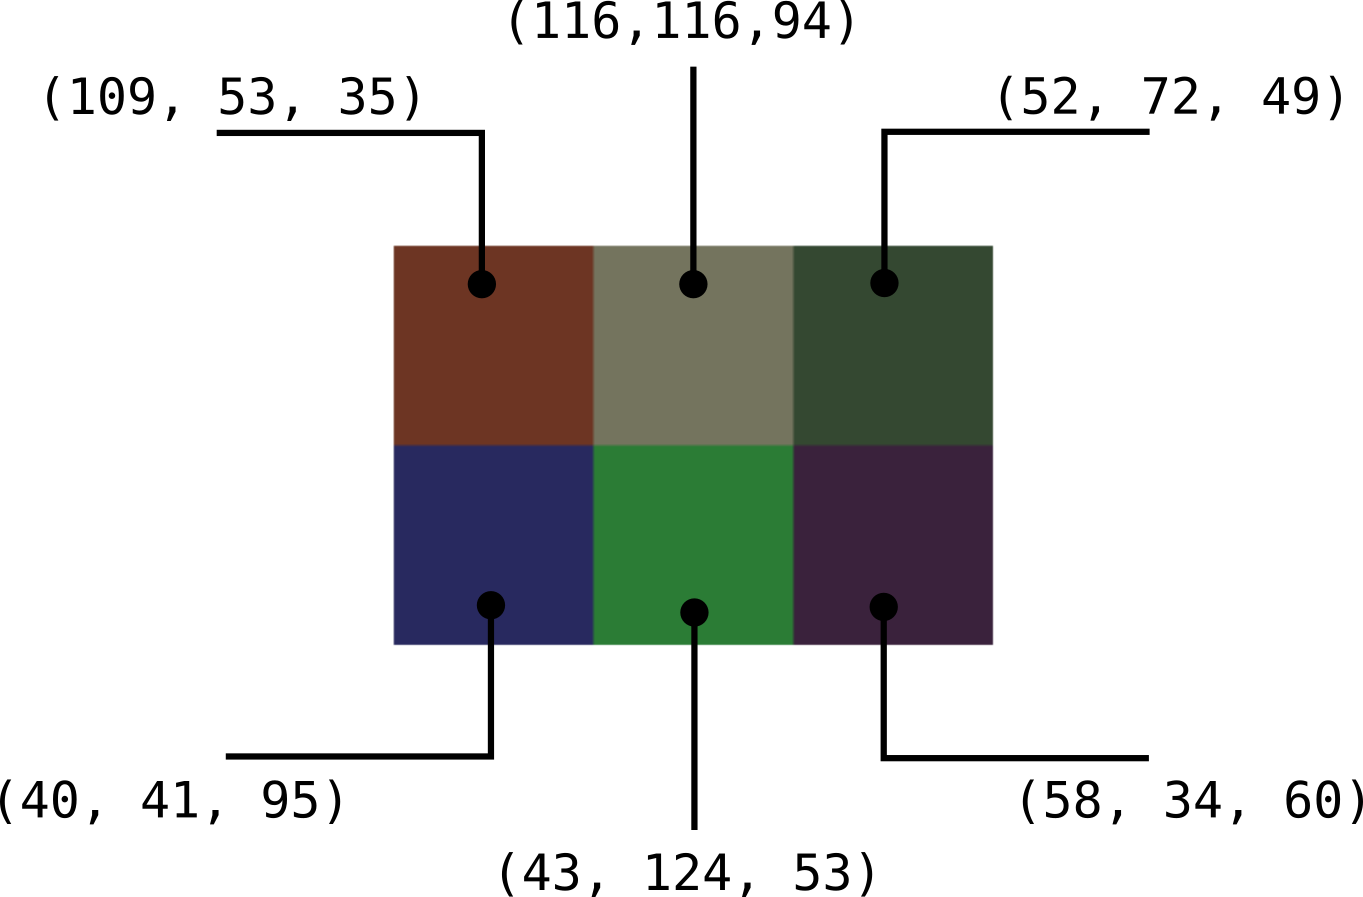
\includegraphics[scale=0.65]{./images/tiny_new_wn.png}
\end{center}
\end{frame}

\begin{frame}[fragile]
\frametitle{Пример изображения}
Ширина = 3 пикселя, высота = 2 пикселя\\
Цвет каждого пикселя кодируется 3-мя байтами\\
\begin{center}
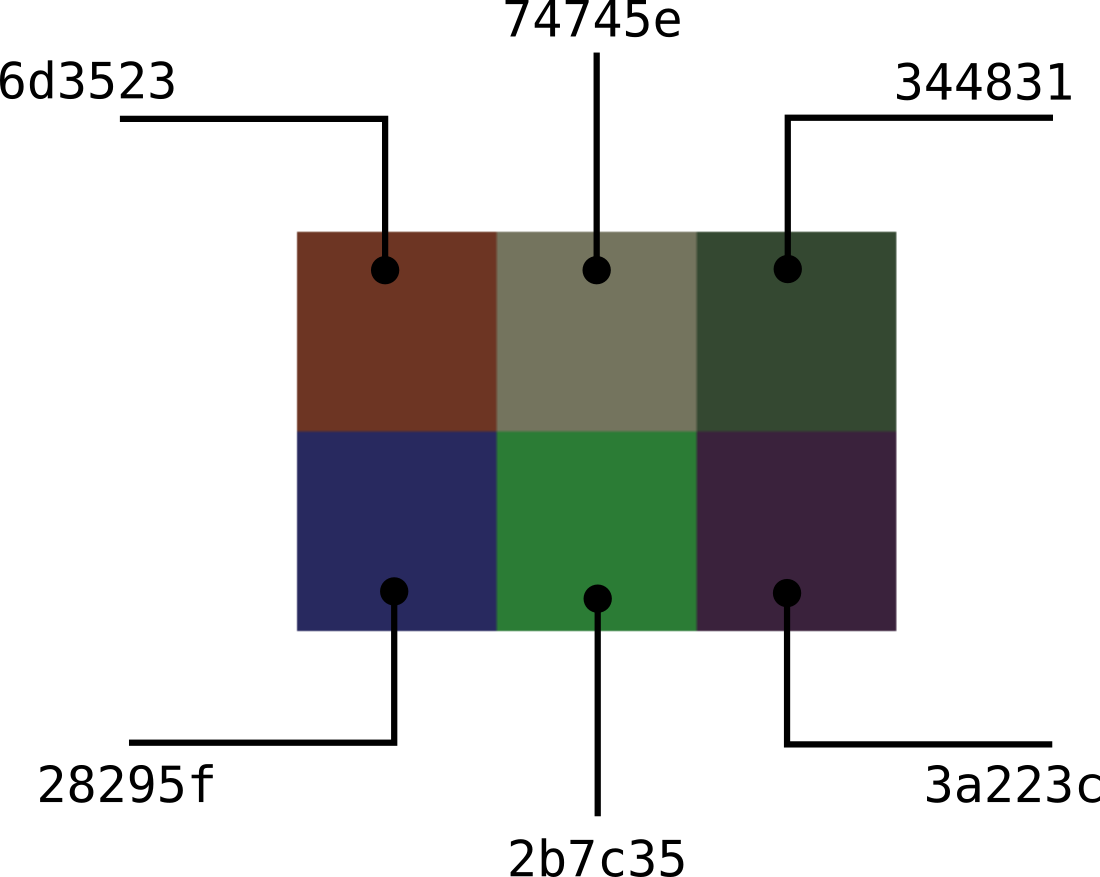
\includegraphics[scale=0.65]{./images/tiny_new_wn_hex.png}
\end{center}
\end{frame}


\begin{frame}[fragile]
\frametitle{Хранение изображения в памяти(стиль C)} 

\begin{center}
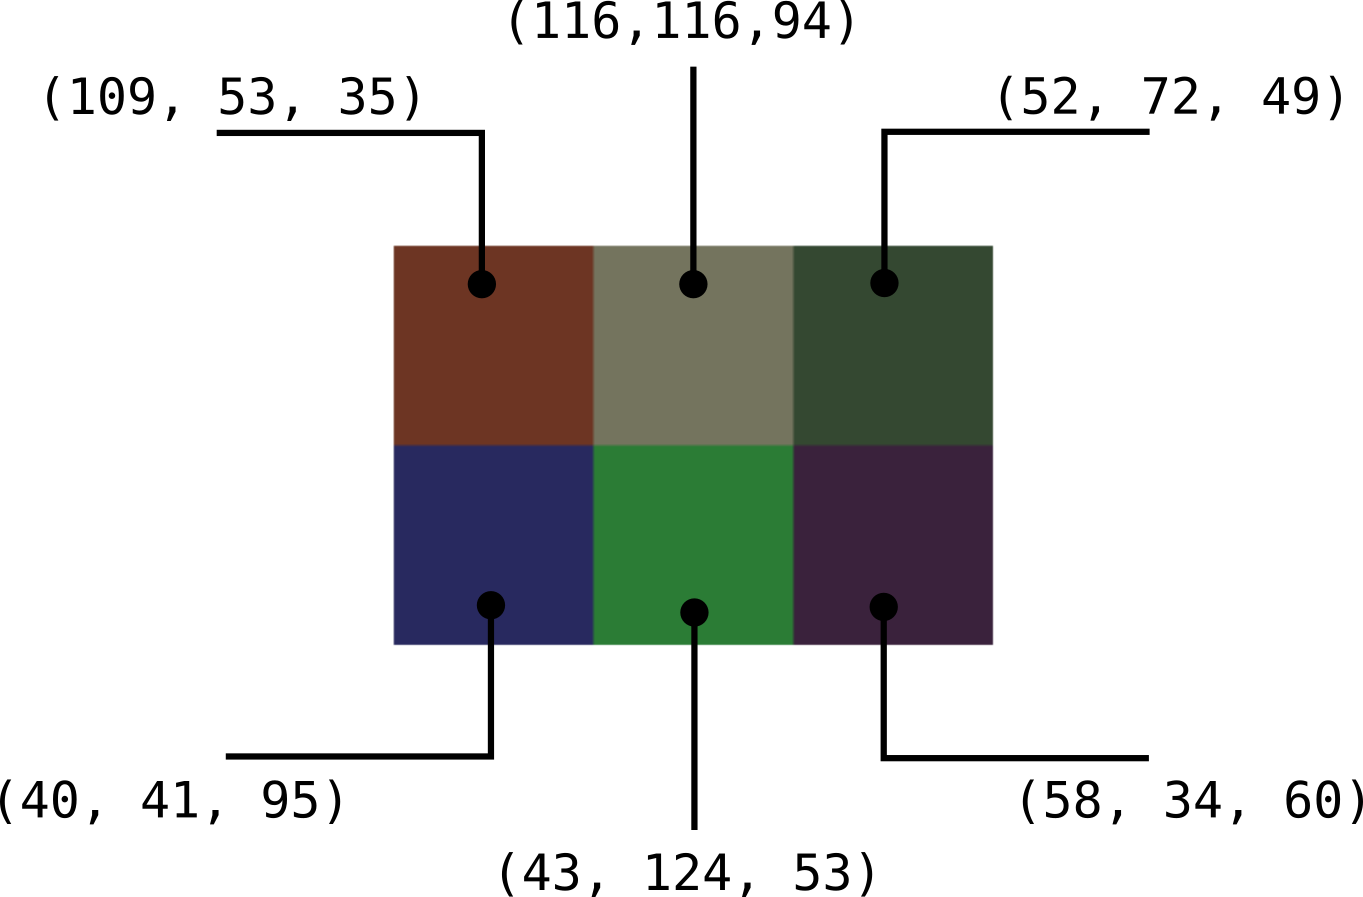
\includegraphics[scale=0.55]{./images/tiny_new_wn.png}
\end{center}

\begin{lstlisting}
int width = 3, height = 2;
unsigned char data[18] = {109, 53, 35, 116, 116, 94, 
                          52, 72, 49, 40, 41, 95,
                          43, 124, 53, 58, 34, 60};
\end{lstlisting}
\end{frame}


\begin{frame}[fragile]
\frametitle{Хранение изображения в памяти(стиль C++)} 

\begin{center}
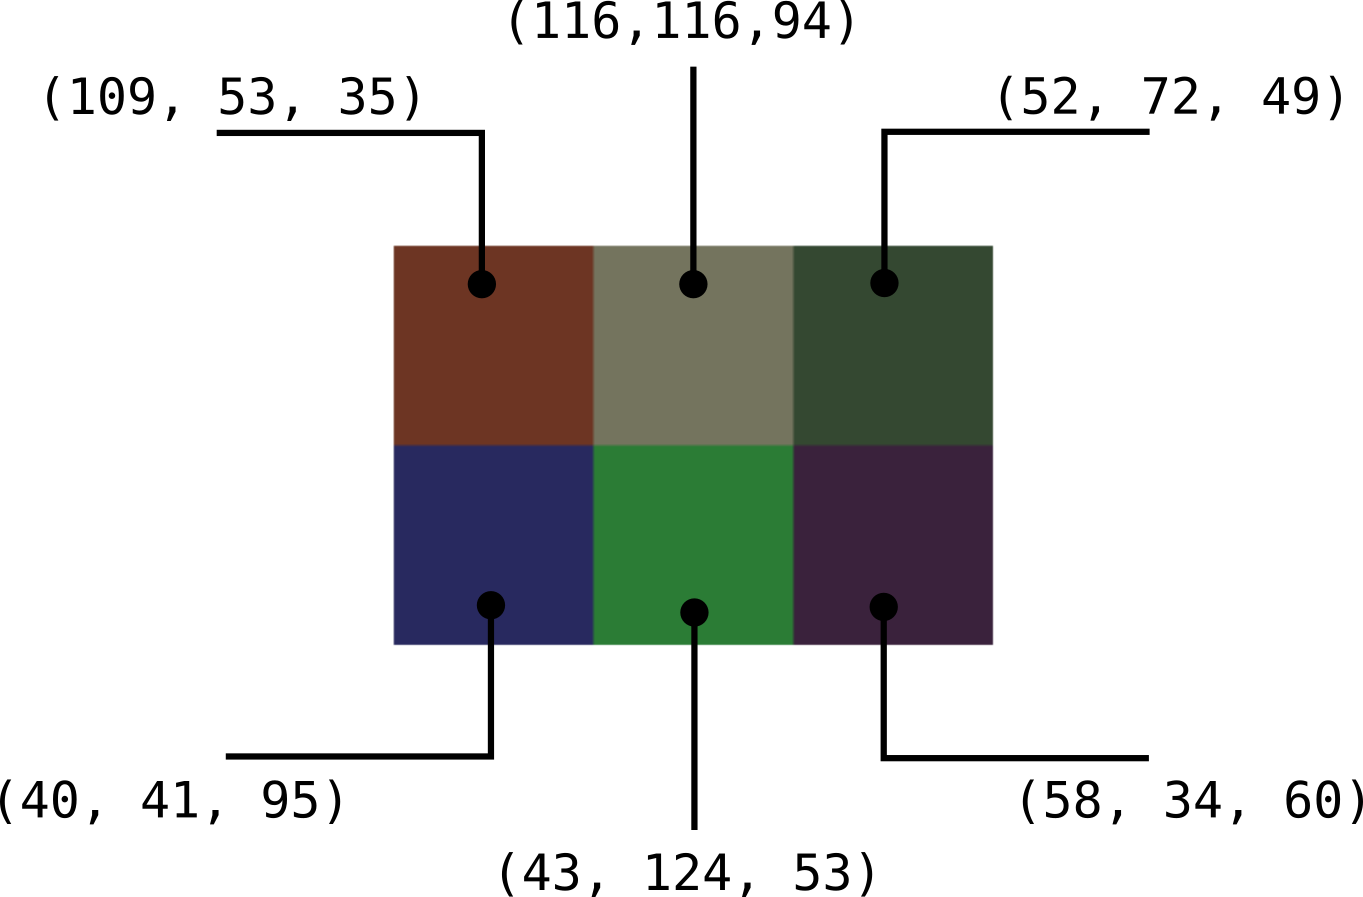
\includegraphics[scale=0.55]{./images/tiny_new_wn.png}
\end{center}

\begin{lstlisting}
int width = 3, height = 2;
std::vector<unsigned char> v {109, 53, 35, 116, 116,94, 
                              52, 72, 49, 40, 41, 95,
                              43, 124, 53, 58, 34, 60};
\end{lstlisting}
\end{frame}


\begin{frame}[fragile]
\frametitle{Хранение изображения в памяти} 

\begin{center}
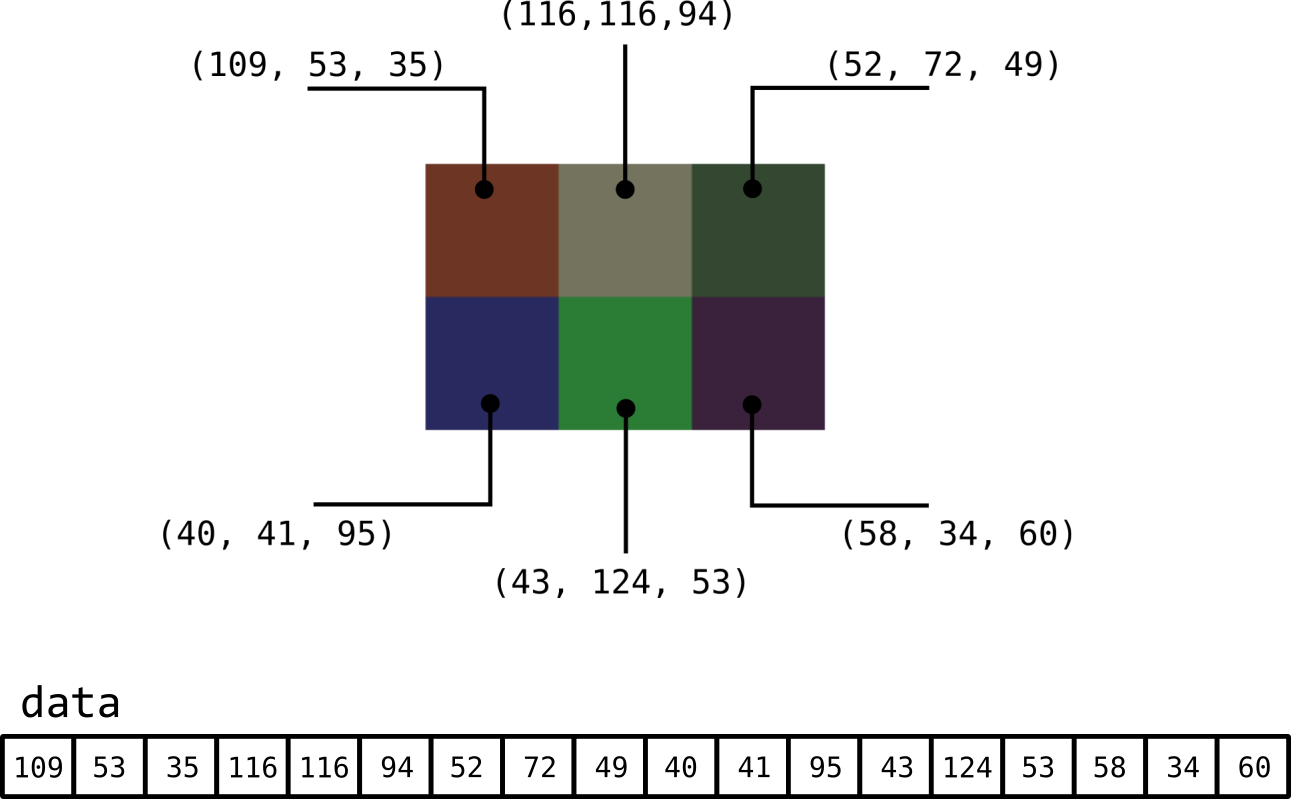
\includegraphics[scale=0.55]{./images/image_in_memory.png}
\end{center}
\end{frame}

\iffalse
\begin{frame}[fragile]
\frametitle{Хранение изображения в памяти (с использованием структуры, представляющей цвет)} 
\begin{lstlisting}
struct Color
{
    unsigned char r, g, b;
};

int main()
{
    int width = 3, height = 2;
    std::vector<Color> v {{109, 53, 35}, {116, 116,94}, 
                          {52, 72, 49},  {40, 41, 95},
                          {43, 124, 53}, {58, 34, 60}};
}
\end{lstlisting}
\end{frame}
\fi


\begin{frame}[fragile]
\frametitle{Координаты пикселей} 
\begin{center}
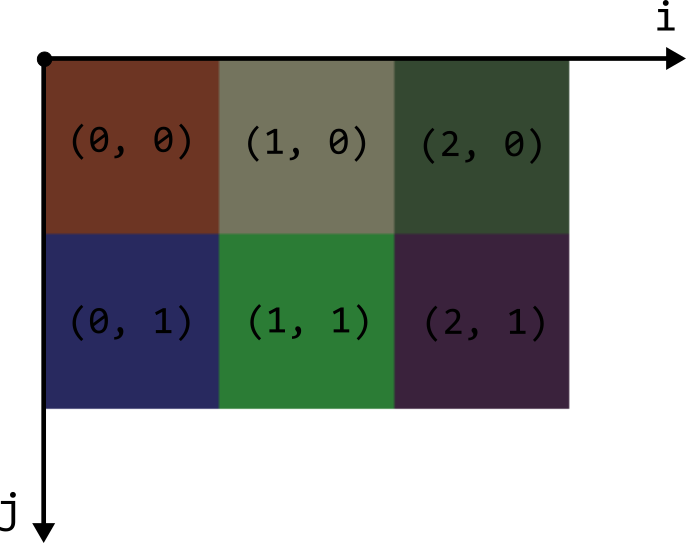
\includegraphics[scale=0.65]{./images/image_coords.png}
\end{center}
\end{frame}

\begin{frame}[fragile]
\frametitle{Индекс компоненты цвета пикселя в массиве} 
\begin{lstlisting}
int width = getImageWidth();
int height = getImageHeight();
std::vector<unsigned char> data = getImageData();
\end{lstlisting}

Изменим \texttt{k}-ю компоненту пикселя с координатами \texttt{(i, j)}:
\begin{lstlisting}
data[3 * (i + j * width) + k] = 100;
\end{lstlisting}
\texttt{i $\in$ [0, width - 1]}, \texttt{j $\in$ [0, height - 1]}, \texttt{k $\in$ [0, 2]},

\begin{center}
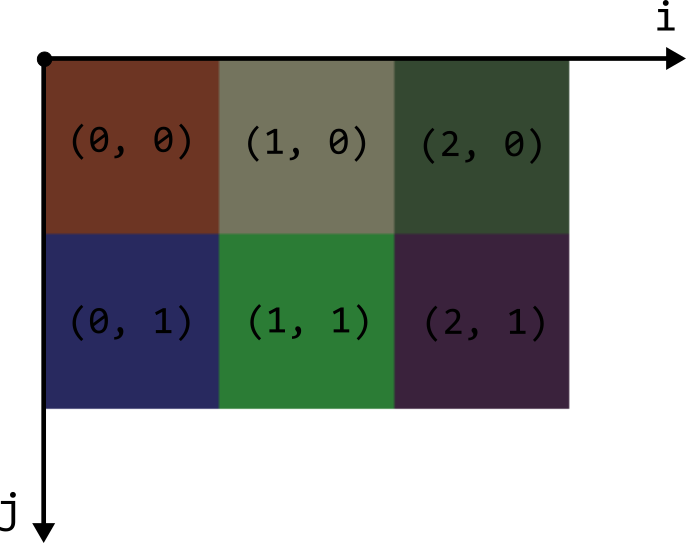
\includegraphics[scale=0.5]{./images/image_coords.png}
\end{center}
\end{frame}


\section{Формат \texttt{.ppm}}

\begin{frame}[fragile]
\frametitle{Пример изображения} 
\begin{center}
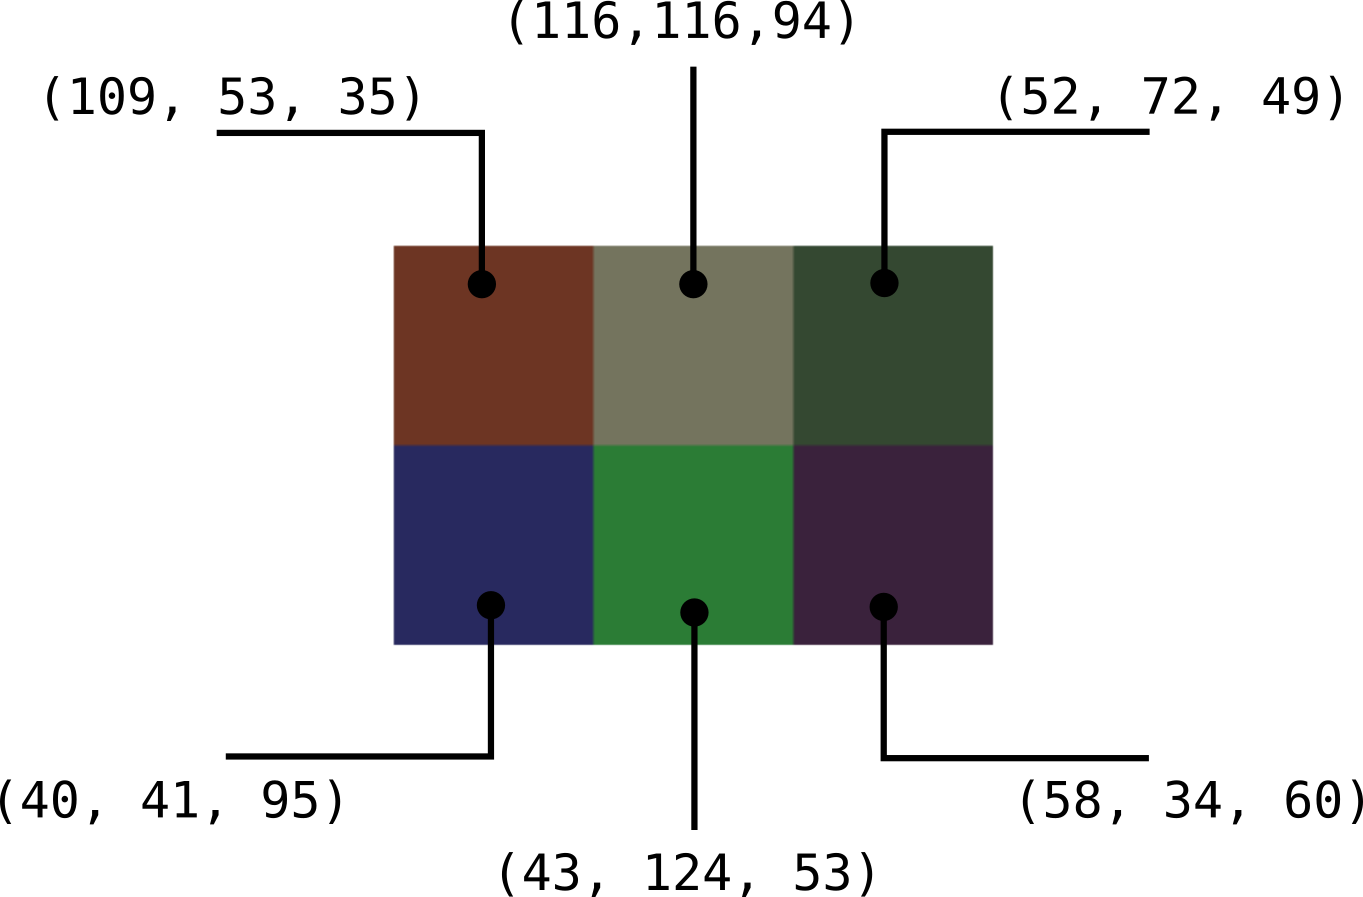
\includegraphics[scale=0.65]{./images/tiny_new_wn.png}
\end{center}
\end{frame}




\begin{frame}[fragile]
\frametitle{Текстовый формат \texttt{.ppm} изображения} 
\begin{multicols}{2}
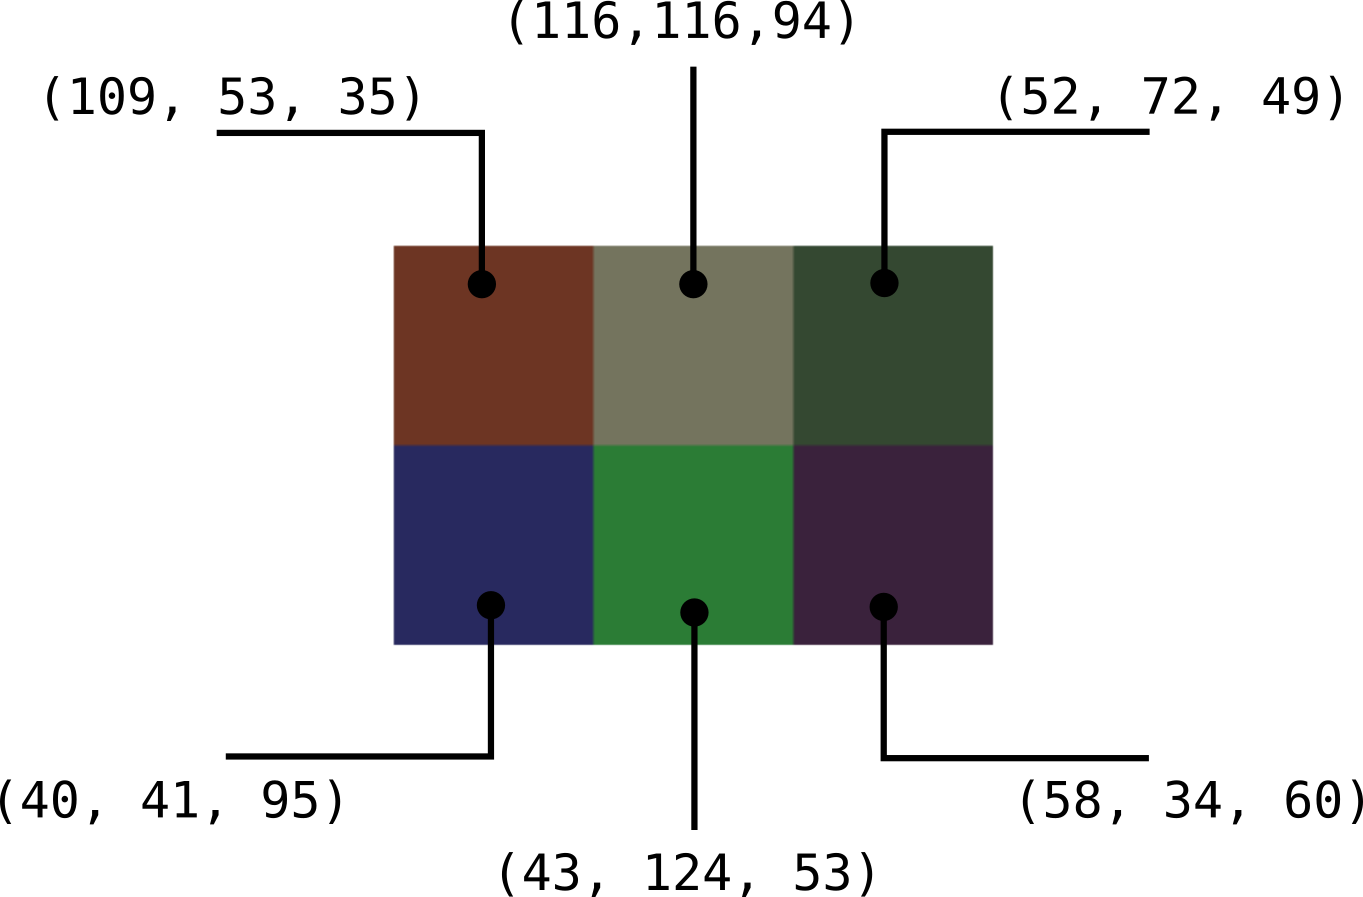
\includegraphics[scale=0.45]{./images/tiny_new_wn.png}
Файл image.ppm
\noindent\fbox{
\parbox{0.4\textwidth}{
\texttt{%
P3\\
3 2\\
255\\
109 53 35 116 116 94 \\
52 72 49 40 41 95 \\
43 124 53 58 34 60
}
}
}
\end{multicols}
\end{frame}

\begin{frame}[fragile]
\frametitle{Текстовый формат \texttt{.ppm} изображения. Побайтово.} 
\begin{multicols}{2}
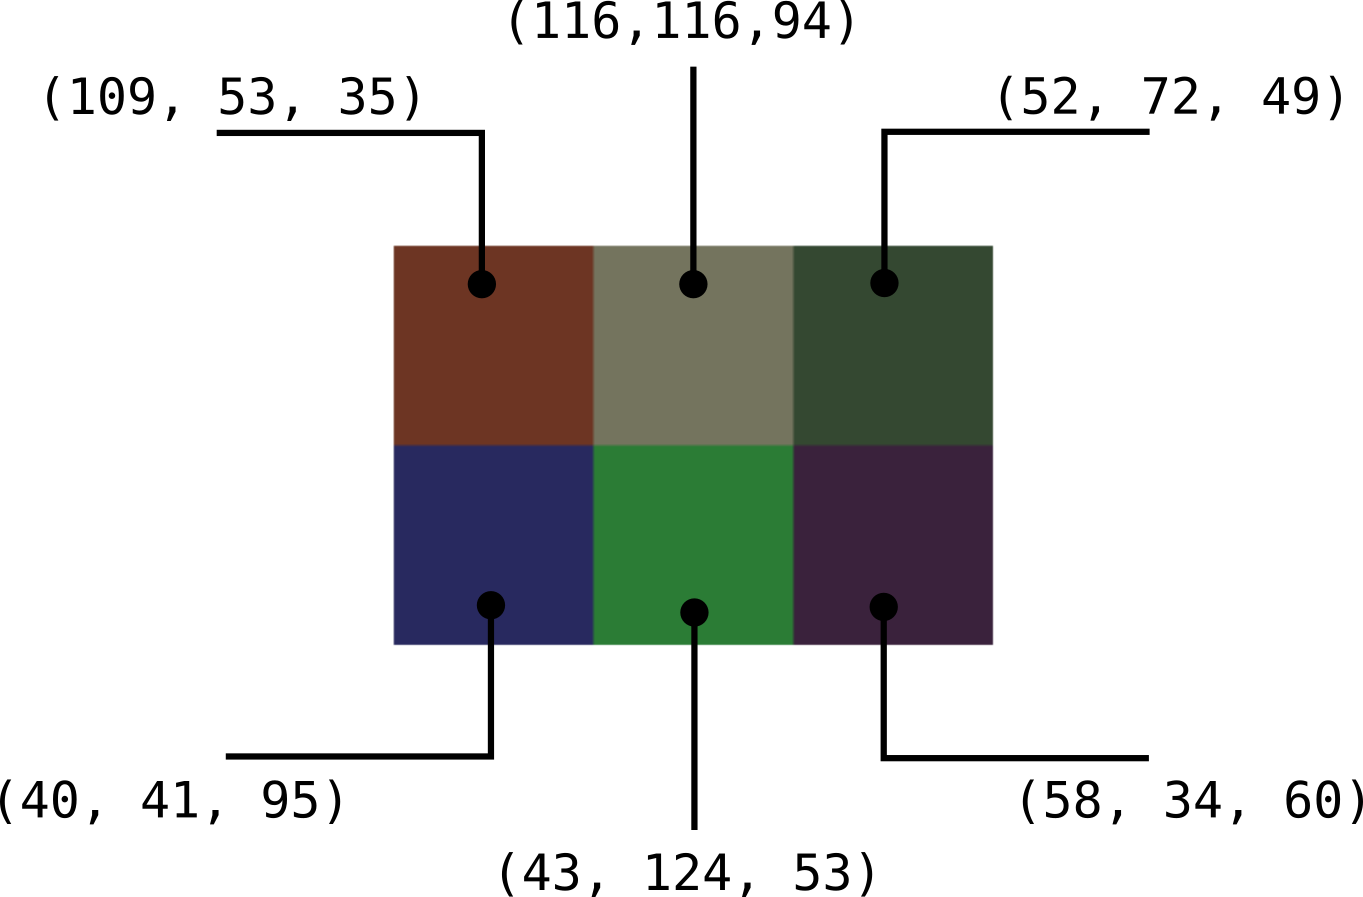
\includegraphics[scale=0.45]{./images/tiny_new_wn.png}
\vfill

\noindent\fbox{
\parbox{0.4\textwidth}{
\texttt{%
50 33 0a 33 20 32 0a 32 \\
35 35 0a 31 30 39 20 35 \\
33 20 33 35 20 0a 31 31 \\
36 20 31 31 36 20 39 34 \\
20 0a 35 32 20 37 32 20 \\
34 39 0a 34 30 20 34 31 \\
20 39 35 20 0a 34 33 20 \\
31 32 34 20 35 33 20 0a \\
35 38 20 33 34 20 36 30 \\
}
}
}
\end{multicols}
\end{frame}



\begin{frame}[fragile]
\frametitle{Запись изображения формата \texttt{ppm P3} } 
\begin{lstlisting}
const int width = 200;
const int height = 100;

std::ofstream out {"my_image.ppm"};
out << "P3\n" << width << " " << height << "\n255\n";

for (int j = 0; j < height; ++j)
{
    for (int i = 0; i < width; ++i)
        out << 40 << " " << 80 << " " << 120 << "\n";
}
\end{lstlisting}
\end{frame}


\begin{frame}[fragile]
\frametitle{Чтение изображения формата \texttt{ppm P3} } 
\begin{lstlisting}
std::ifstream in {"my_file.ppm"};

std::string type;
in >> type;
if (type != "P3")
{
    std::cout << "Error. Format should be P3\n";
    std::exit(1);
}

int width, height, maxValue; 
in >> width >> height >> maxValue;
...
\end{lstlisting}
\end{frame}

\begin{frame}[fragile]
\frametitle{Чтение изображения формата \texttt{ppm P3} } 
\begin{lstlisting}
...
std::vector<unsigned char> data(width * height);

for (int j = 0; j < height; ++j) 
{
    for (int i = 0; i < width; ++i) 
    {
        int ri, gi, bi;
        in >> r >> g >> b;
        unsigned char r = ri, g = gi, b = bi;
        data[3 * (j * width + i) + 0] = r;
        data[3 * (j * width + i) + 1] = g;
        data[3 * (j * width + i) + 2] = b;
     }
}
\end{lstlisting}
\end{frame}


\begin{frame}[fragile]
\frametitle{Варианты формата \texttt{ppm}.} 
\begin{itemize}
\item \texttt{P1}: На каждый пиксель приходится 1 бит   информации
\item \texttt{P2}: На каждый пиксель приходится 1 байт  информации
\item \texttt{P3}: На каждый пиксель приходится 3 байта информации
\item \texttt{P4}: То же самое, что и \texttt{P1}, но в бинарном формате
\item \texttt{P5}: То же самое, что и \texttt{P2}, но в бинарном формате
\item \texttt{P6}: То же самое, что и \texttt{P3}, но в бинарном формате
\end{itemize}
\end{frame}


\begin{frame}[fragile]
\frametitle{Бинарный формат \texttt{.ppm} изображения} 
\begin{multicols}{2}
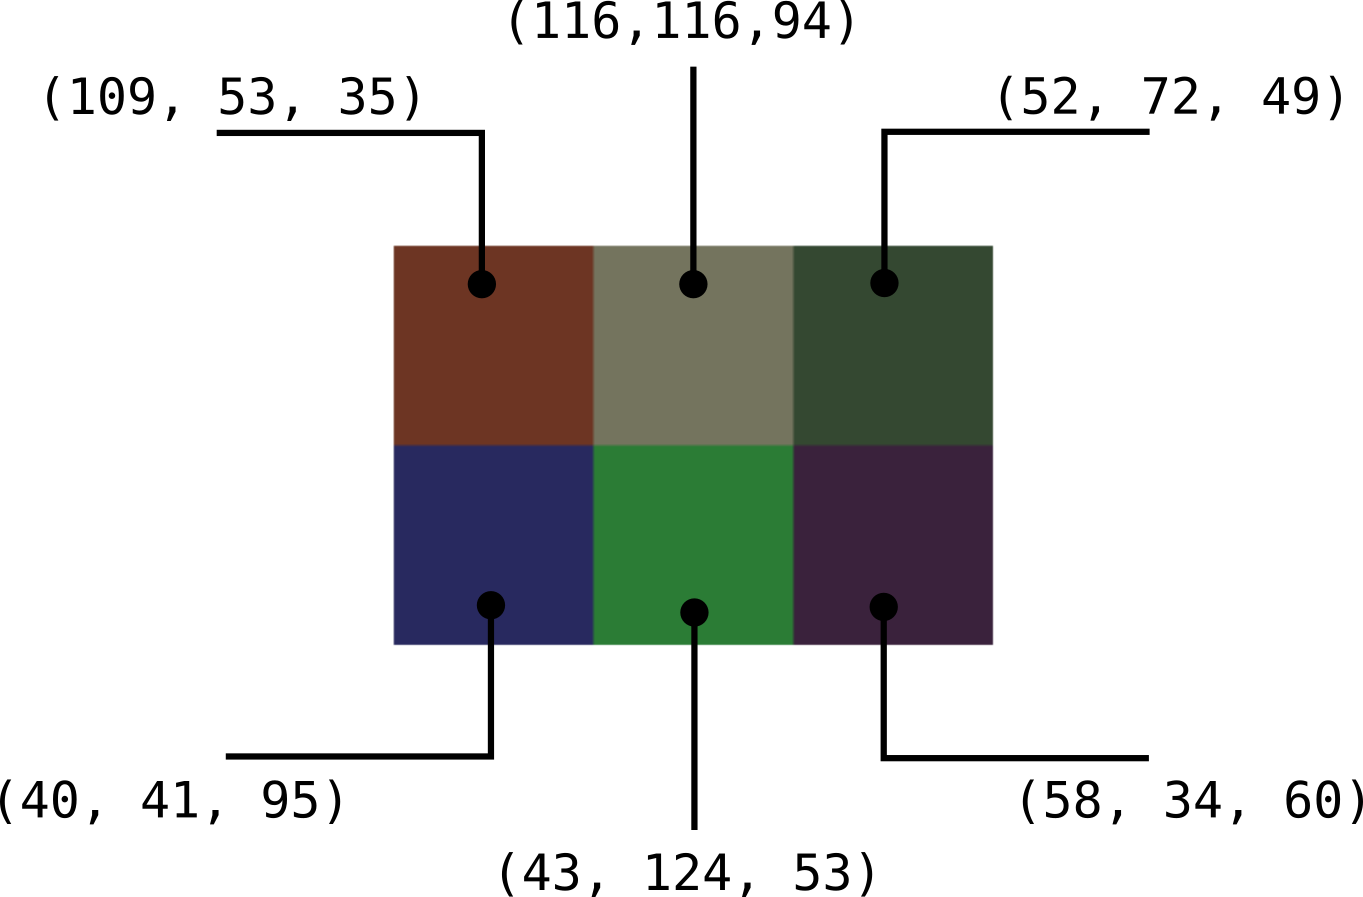
\includegraphics[scale=0.45]{./images/tiny_new_wn.png}
\vfill
Если изображение открыть в текстовом редакторе:
\noindent\fbox{
\parbox{0.4\textwidth}{
\texttt{%
P6\\
3 2\\
255\\
m5\#tt\textasciicircum4H1()\_+|5:"<
}
}
}
\end{multicols}
\end{frame}


\begin{frame}[fragile]
\frametitle{Бинарный формат \texttt{.ppm} изображения. Побайтово.} 
\begin{multicols}{2}
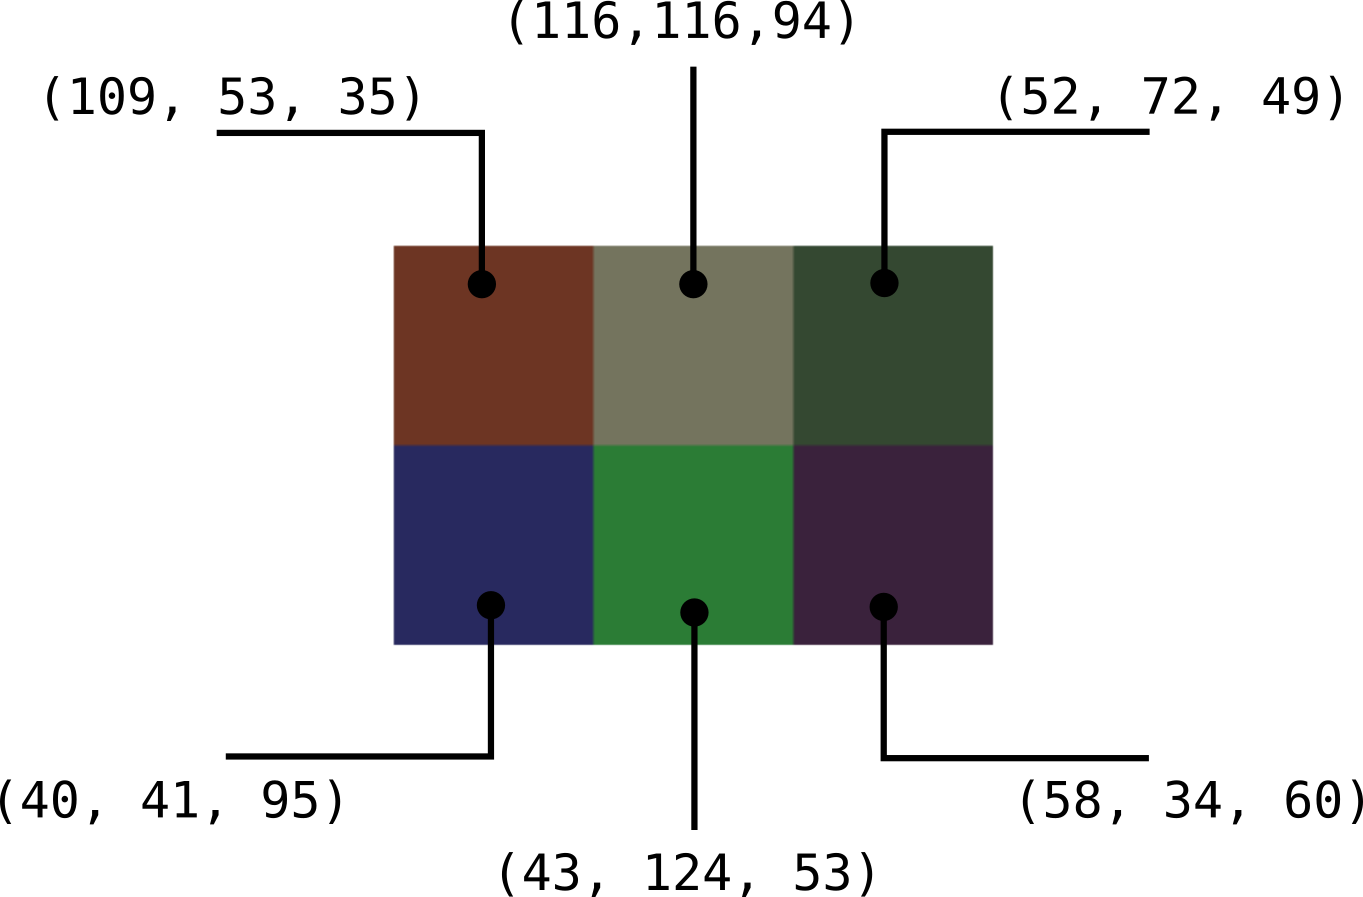
\includegraphics[scale=0.45]{./images/tiny_new_wn.png}

\vfill
Байты файла изображения:
\noindent\fbox{
\parbox{0.4\textwidth}{
\texttt{%
50 36 0a 33 20 32 0a 32 \\ 
35 35 0a 6d 35 23 74 74 \\ 
5e 34 48 31 28 29 5f 2b \\
7c 35 3a 22 3c
}
}
}
\end{multicols}
\end{frame}


\begin{frame}[fragile]
\frametitle{Бинарный формат \texttt{.ppm} изображения. Побайтово.} 
\begin{multicols}{2}
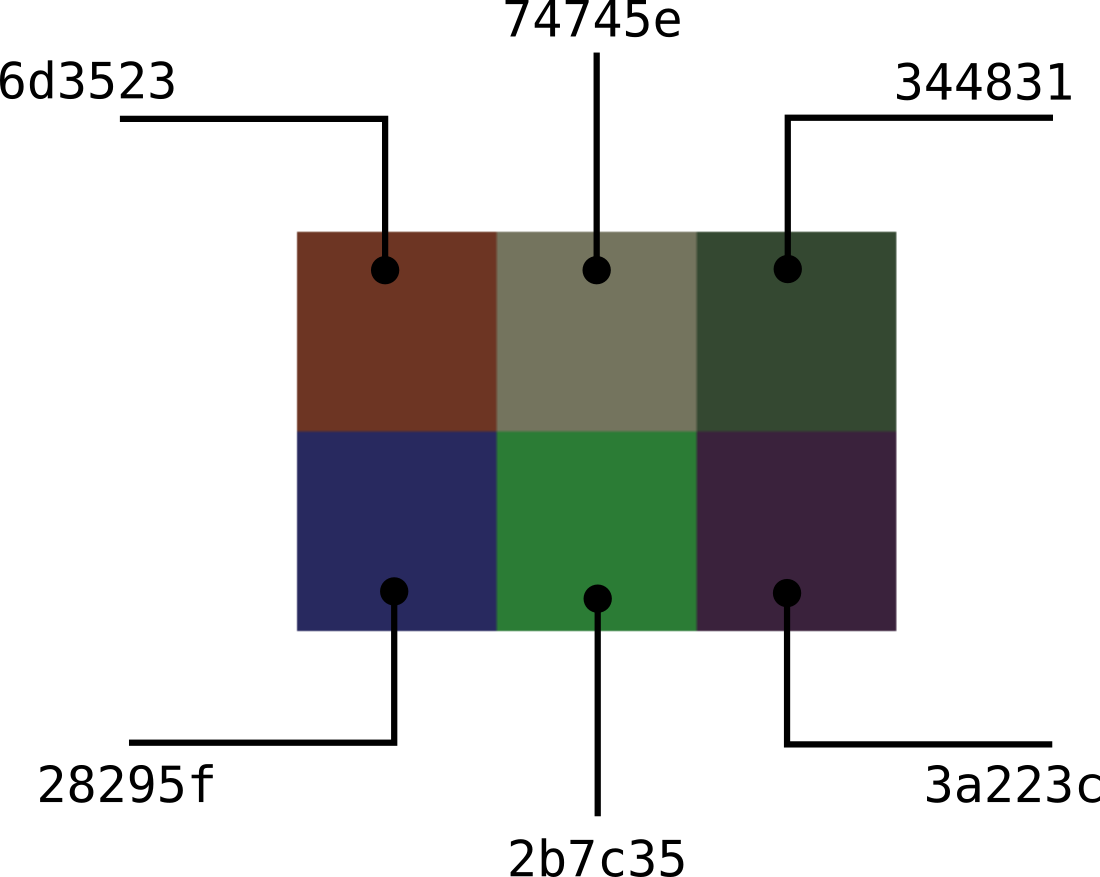
\includegraphics[scale=0.45]{./images/tiny_new_wn_hex.png}

\vfill
Байты файла изображения:
\noindent\fbox{
\parbox{0.4\textwidth}{
\texttt{%
50 36 0a 33 20 32 0a 32 \\ 
35 35 0a 6d 35 23 74 74 \\ 
5e 34 48 31 28 29 5f 2b \\
7c 35 3a 22 3c
}
}
}
\end{multicols}
\end{frame}


\begin{frame}[fragile]
\frametitle{Запись изображения формата \texttt{ppm P6} } 
\begin{lstlisting}
const int width = getWidth();
const int height = getHeight();
std::vector<unsigned char> data = getData();

std::ofstream out {"result.ppm", std::ios::binary};

out << "P6\n" << width << " " << height << "\n255\n";

out.write(reinterpret_cast<const char*>(&data[0]), data.size());
\end{lstlisting}
\end{frame}


\begin{frame}[fragile]
\frametitle{Чтение изображения формата \texttt{ppm P6} } 
\begin{lstlisting}
std::ifstream in {"image.ppm", std::ios::binary};
if (in.fail()) 
{
    std::cout << "Error. Can't open file!\n";
    std::exit(1);
}

std::string type;
in >> type;
if (type != "P6") 
{
    std::cout << "Error. File should be type P6\n";
    std::exit(1);
}
...
\end{lstlisting}
\end{frame}


\begin{frame}[fragile]
\frametitle{Чтение изображения формата \texttt{ppm P6} } 
\begin{lstlisting}
...
int width, height, maxValue;
in >> width >> height >> in >> maxValue;

char temp;
in >> std::noskipws >> temp;

std::vector<unsigned char> data(3 * width * height);
in.read(reinterpret_cast<char*>(&data[0]), data.size());
\end{lstlisting}
\end{frame}

\section{Формат \texttt{jpeg}}

\begin{frame}[fragile]
\frametitle{Конверсия из \texttt{RGB} в \texttt{YCbCr}} 
\begin{center}
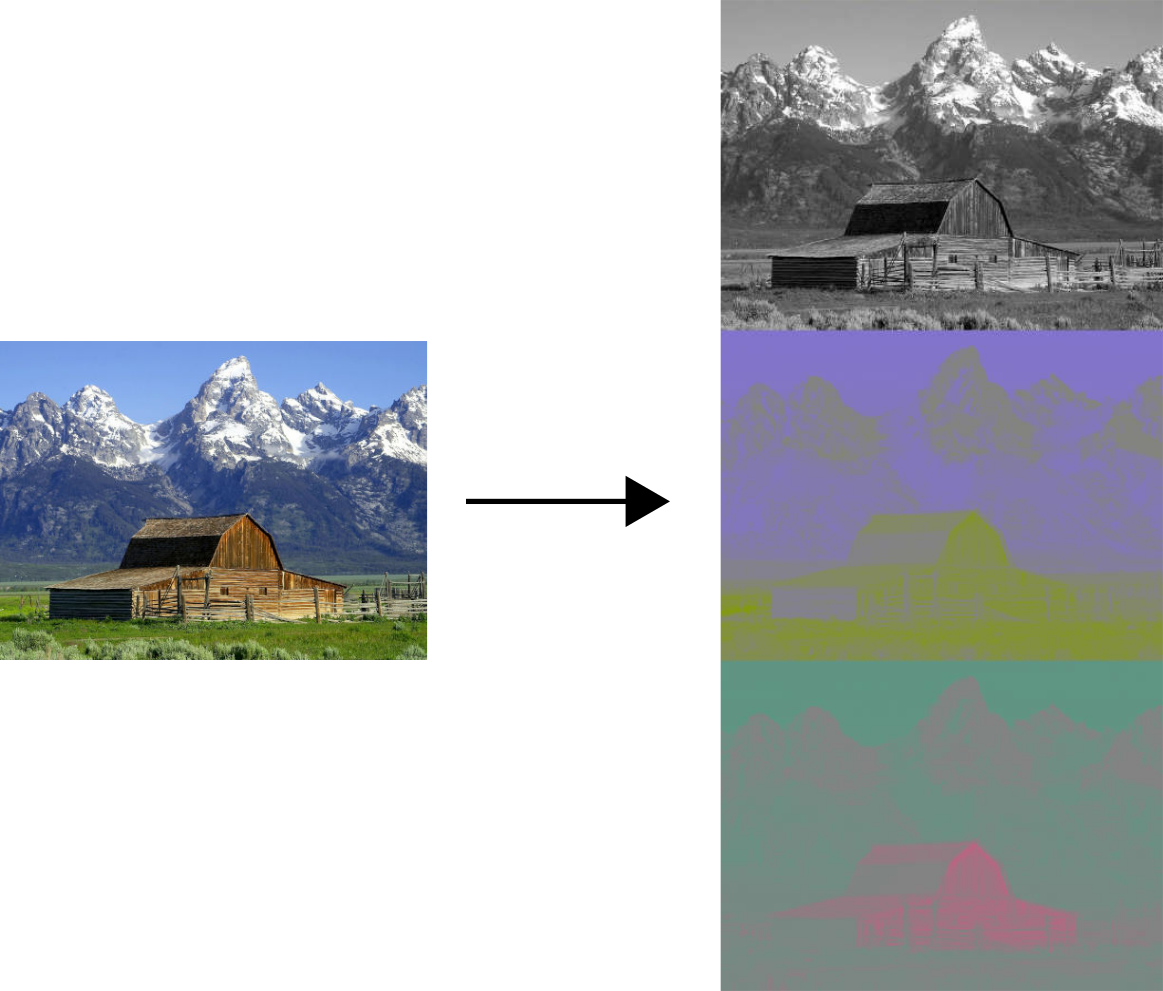
\includegraphics[scale=0.4]{./images/rgb_to_ycbcr.png}
\end{center}
\end{frame}

\begin{frame}[fragile]
\frametitle{Конверсия из \texttt{RGB} в \texttt{YCbCr}}

\begin{enumerate}
\item Перевод из \texttt{RGB} в \texttt{YCbCr}:
\begin{align*}
y  &= 0.299 \cdot r + 0.587 \cdot g + 0.114 \cdot b \\
cb &= 128 - 0.169 \cdot r - 0.331 \cdot g + 0.5 \cdot b \\
cr &= 128 + 0.5 \cdot r - 0.419 \cdot g - 0.081 \cdot b \\
\end{align*}

\item Downsampling компонент \texttt{Cb} и \texttt{Cr}
\end{enumerate}

\end{frame}

\begin{frame}[fragile]
\frametitle{Дискретное косинусное преобразование} 

\begin{enumerate}
\setcounter{enumi}{2}
\item Разбиваем изображение на блоки 8 на 8 пикселей.
\item Проводим дискретное косинусное преобразование для каждого блока.
\end{enumerate}

Базис разложения:
\begin{center}
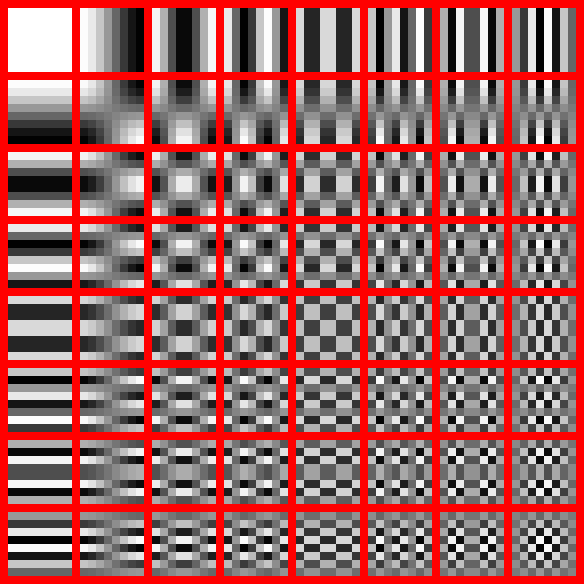
\includegraphics[scale=0.26]{./images/dctjpeg.png}
\end{center}
\end{frame}

\begin{frame}[fragile]
\frametitle{Дискретное косинусное преобразование} 
\begin{enumerate}
\setcounter{enumi}{4}
\item Для каждого блока 8 на 8 получится матрица примерно такого вида:
\end{enumerate}
\begin{center}
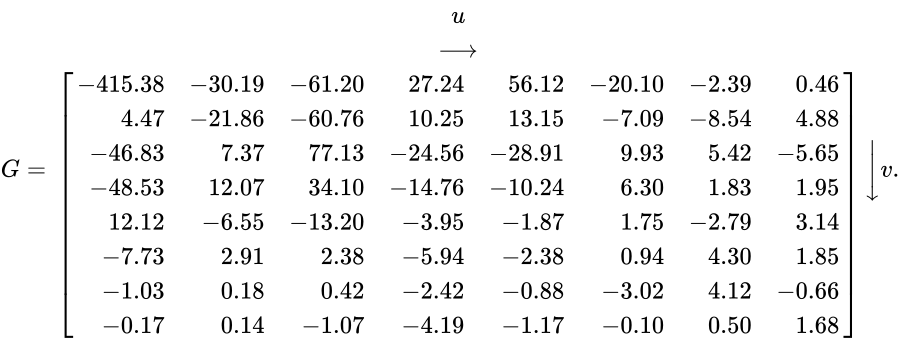
\includegraphics[scale=0.45]{./images/matrix1.png}
\end{center}
\end{frame}


\begin{frame}[fragile]
\frametitle{Квантизация} 
\begin{enumerate}
\setcounter{enumi}{5}
\item Делим каждый элемент матрицы на элемент матрицы квантизации $Q$.
Получится матрица $B$.
\end{enumerate}
\begin{center}
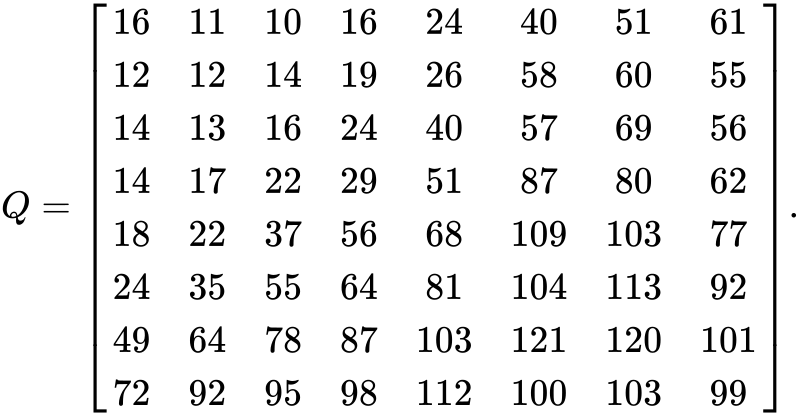
\includegraphics[scale=0.26]{./images/matrix2.png}
\end{center}

\begin{center}
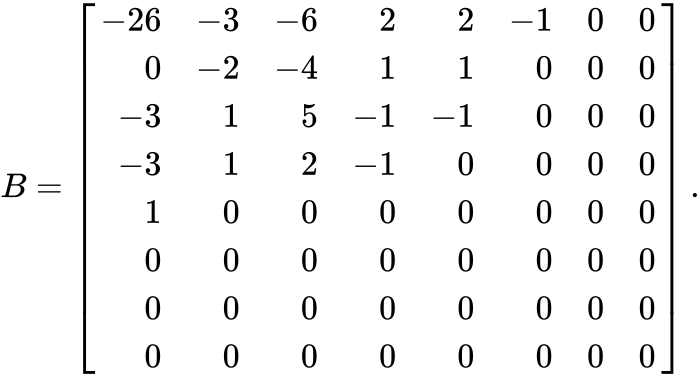
\includegraphics[scale=0.26]{./images/matrix3.png}
\end{center}
\end{frame}


\begin{frame}[fragile]
\frametitle{Сжатие} 
\begin{enumerate}
\setcounter{enumi}{6}
\item Сохраняем матрицу $B$ зигзагом, чтобы нули были сгруппированы.
\item Сжимаем полученные данные с помощью кода Хаффмана.
\end{enumerate}
\begin{center}
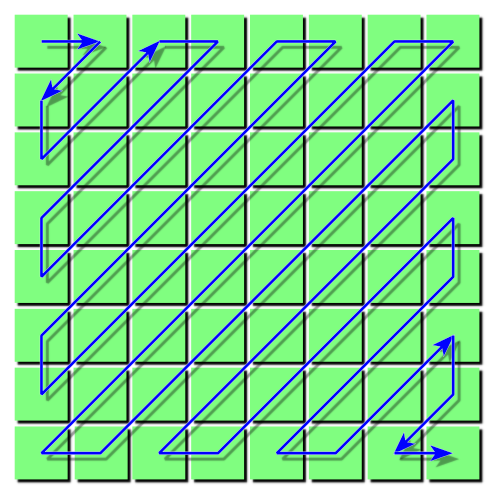
\includegraphics[scale=0.4]{./images/jpeg_zigzag.png}
\end{center}
\end{frame}


\begin{frame}[fragile]
\frametitle{Сжатие} 
\begin{center}
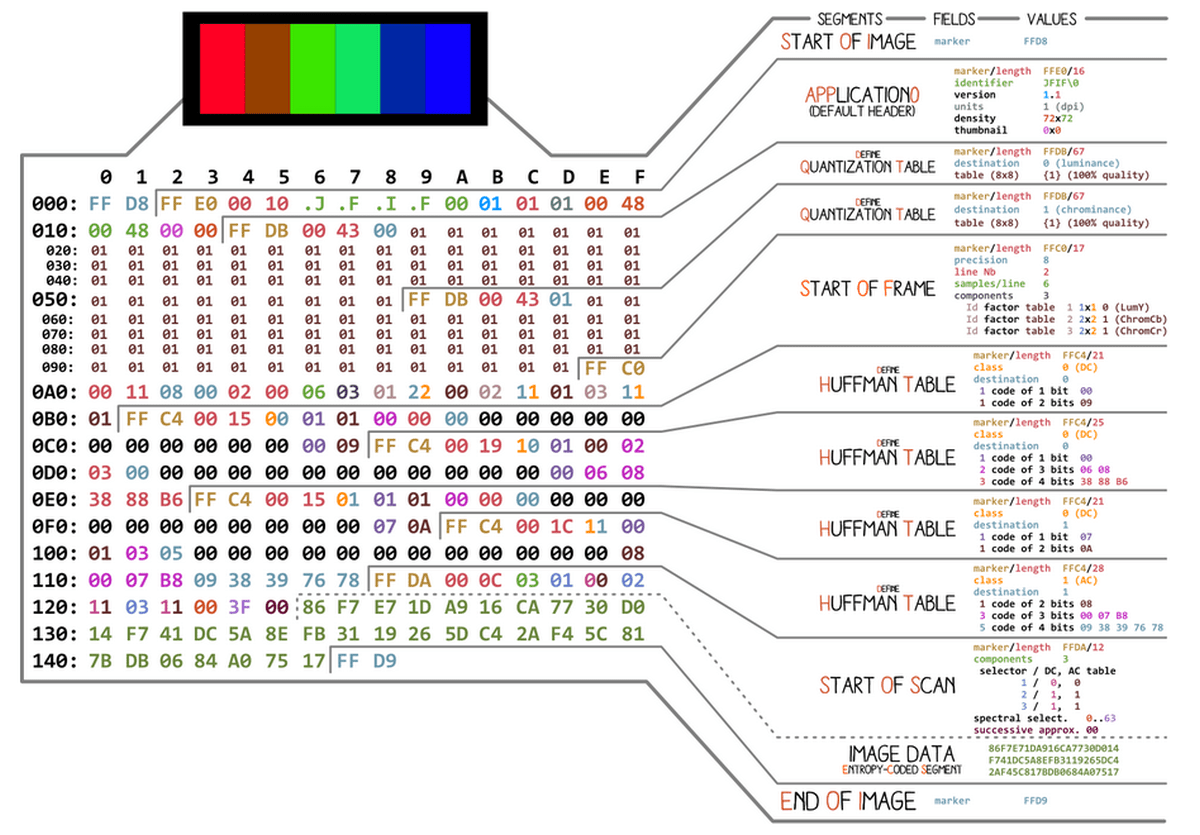
\includegraphics[scale=0.6]{./images/050.png}
\end{center}
\end{frame}

\begin{frame}[fragile]
\frametitle{Библиотека stb} 

Библиотеку stb можно найти в \texttt{https://github.com/nothings/stb}

\begin{itemize}
\item \texttt{stb\_image.h} библиотека для чтения изображения в форматах JPG, PNG, GIF, BMP и других.
\begin{lstlisting}
#define STB_IMAGE_IMPLEMENTATION
#include "stb_image.h"
\end{lstlisting}

\item \texttt{stb\_image\_write.h} библиотека для чтения изображения в форматах JPG, PNG, GIF, BMP и других.
\begin{lstlisting}
#define STB_IMAGE_WRITE_IMPLEMENTATION
#include "stb_image_write.h"
\end{lstlisting}
\end{itemize}
\end{frame}

\begin{frame}[fragile]
\frametitle{Чтение изображения формата \texttt{jpeg} с помощью библиотеки stb} 
\begin{lstlisting}
int width, height, channels;
unsigned char* img = stbi_load("russian_peasants.jpg", &width, &height, &channels, 0);
    
if(img == NULL)
{
     std::cout << "Error while loading image\n";
     exit(1);
}
\end{lstlisting}
\end{frame}


\begin{frame}[fragile]
\frametitle{Запись изображения формата \texttt{jpeg} с помощью библиотеки stb} 
\begin{lstlisting}
int width = 400, height = 300, channels = 3;
std::vector<unsigned char> v = ...;

int success = stbi_write_jpg("test.jpg", width, height, channels, v.data, 100);
if(success == 0)
{
    std::cout << "Error while saving image\n";
    exit(1);
}
\end{lstlisting}
\end{frame}


\section*{Создаём класс изображения}

\begin{frame}[fragile]
\frametitle{Класс \texttt{Image}} 
\begin{lstlisting}
class Image
{
private:
    int mWidth  {0};
    int mHeight {0};
    std::vector<unsigned char> mData {};
public:
    Image() {}
    Image(const std::string& filename);
    Image(int width, int height);
    Image(int width, int height, Color c);

    int getWidth();
    int getHeight();
    unsigned char* getData();
    ...
\end{lstlisting}
\end{frame}

\begin{frame}[fragile]
\frametitle{Класс \texttt{Image}} 
\begin{lstlisting}
    ...
    void setPixel(int i, int j, Color c);
    Color getPixel(int i, int j) const;

    Color& operator()(int i, int j);

    void loadPPMText(const std::string& fn);
    void savePPMText(const std::string& fn) const;
    void loadPPMBinary(const std::string& fn);
    void savePPMBinary(const std::string& fn) const;
    void loadPPM(const std::string& fn);
    void loadJPEG(const std::string& fn);
    void saveJPEG(const std::string& fn) const;
}
\end{lstlisting}
\end{frame}

\begin{frame}[fragile]
\frametitle{Класс \texttt{Image}. Вспомательный класс \texttt{Color}} 
\begin{lstlisting}
class Image
{
public:

struct Color
{
    unsigned char r, g, b;

    Color& operator+=(const Color& c);
    Color operator+(const Color& c) const;
};

...

}
\end{lstlisting}
\end{frame}


\begin{frame}[fragile]
\frametitle{Работа с классом \texttt{Image}.} 
\begin{lstlisting}
Image a {"input.ppm"};

for (int j = 0; j < a.getHeight(); ++j)
{
    for (int i = 0; i < a.getWidth(); ++i)
        a(i, j) += Image::Color{20, 20, 20};
}

b.savePPMBinary("output.ppm");
\end{lstlisting}
\end{frame}


\section*{Рисование на изображении. Алгоритм Брезенхема.}

\begin{frame}[fragile]
\frametitle{Рисуем прямоугольник} 
\begin{lstlisting}
Image a {"input.ppm"};

for (int j = 300; j < 400; ++j)
{
    for (int i = 100; i < 300; ++i)
        a(i, j) = Image::Color{255, 0, 0};
}

b.savePPMBinary("output.ppm");
\end{lstlisting}
\end{frame}


\begin{frame}[fragile]
\frametitle{Как нарисовать линию?} 
\begin{center}
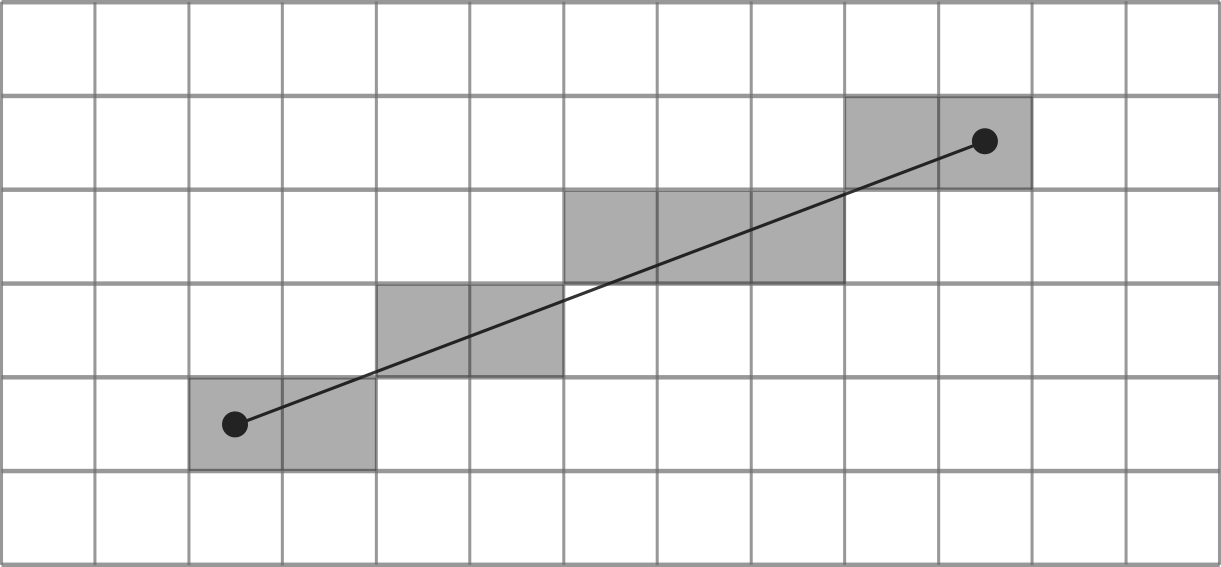
\includegraphics[scale=0.75]{./images/bresenham.png}
\end{center}
\end{frame}


\begin{frame}[fragile]
\frametitle{Как нарисовать линию?} 
$$
y = \frac{y_1 - y_0}{x_1 - x_0} (x - x_0) + y_0
$$
\begin{center}
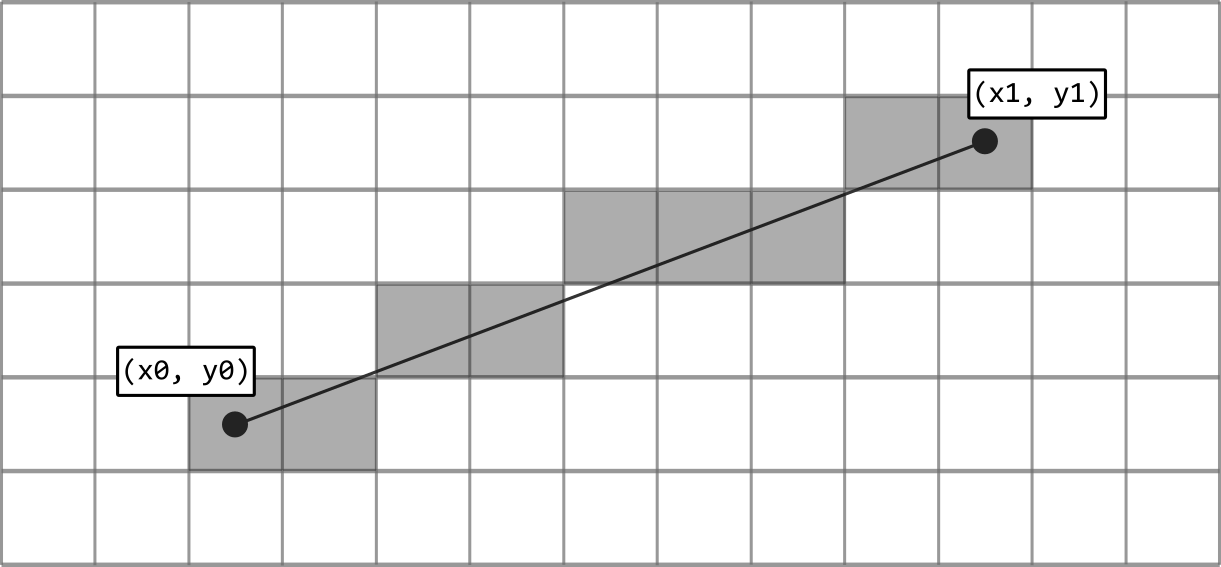
\includegraphics[scale=0.75]{./images/bresenham_xy.png}
\end{center}
\end{frame}



\begin{frame}[fragile]
\frametitle{Рисуем линию (углы от -45 до +45 градусов с Ox)} 
\begin{lstlisting}
void line(Image& im, int x0, int y0, int x1, int y1) {
    int dx = abs(x1 - x0), dy = abs(y1 - y0);
    int diry = y1 - y0;
    if (diry > 0) diry = 1; 
    if (diry < 0) diry = -1;

    int y = y0, error = 0;
    for (int x = x0; x < x1; ++x) {
        im(x, y) = Image::Color{0, 0, 0};
        error += dy;
        if (error >= dx) {
            y += diry;
            error -= dx;
        }
    }
}
\end{lstlisting}
\end{frame}


\begin{frame}[fragile]
\frametitle{Антиалиасинг} 
\begin{center}

\includegraphics[scale=0.4]{./images/anti-aliasing.png}
\end{center}
\end{frame}

\begin{frame}[fragile]
\frametitle{Алгоритмы для устранения антиалиасинга} 
\begin{itemize}
\item Алгоритм Ву\\
\begin{center}
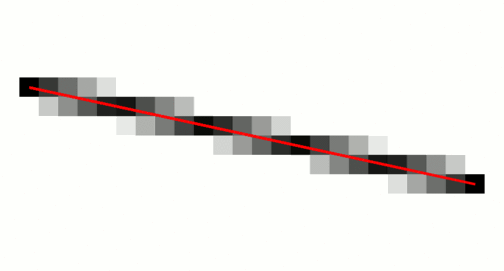
\includegraphics[scale=0.26]{./images/wu.png}
\end{center}
\item Supersampling
\begin{multicols}{2}
\begin{center}
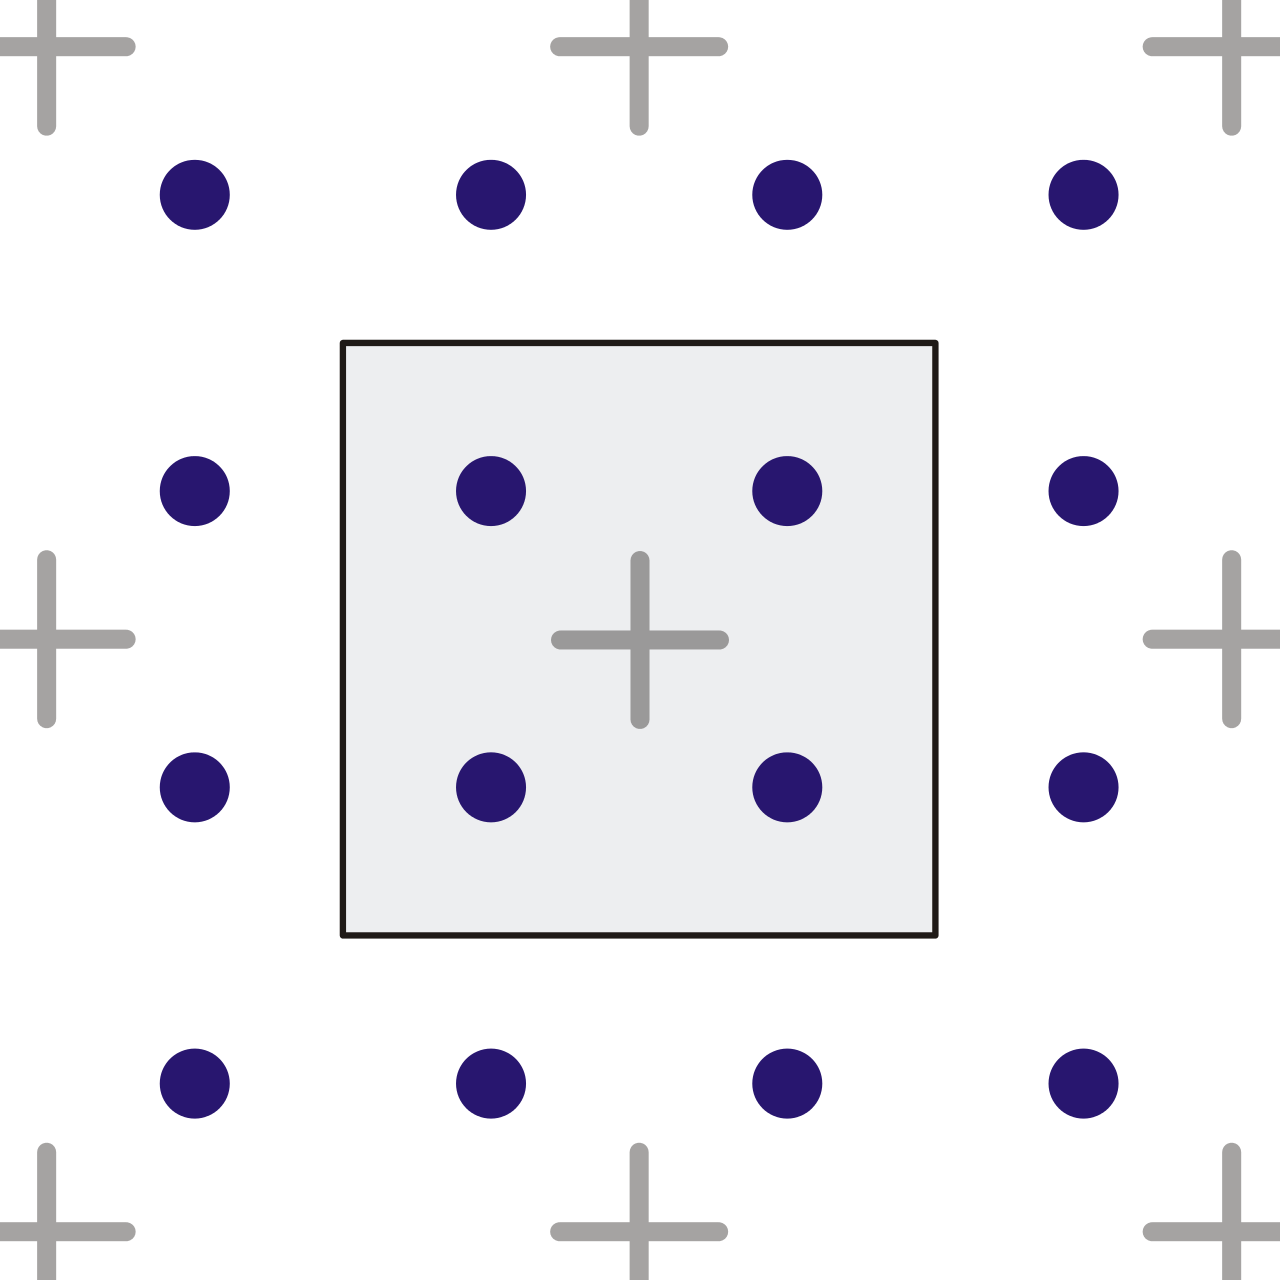
\includegraphics[scale=0.05]{./images/supersampling1.png}
\end{center}
\begin{center}
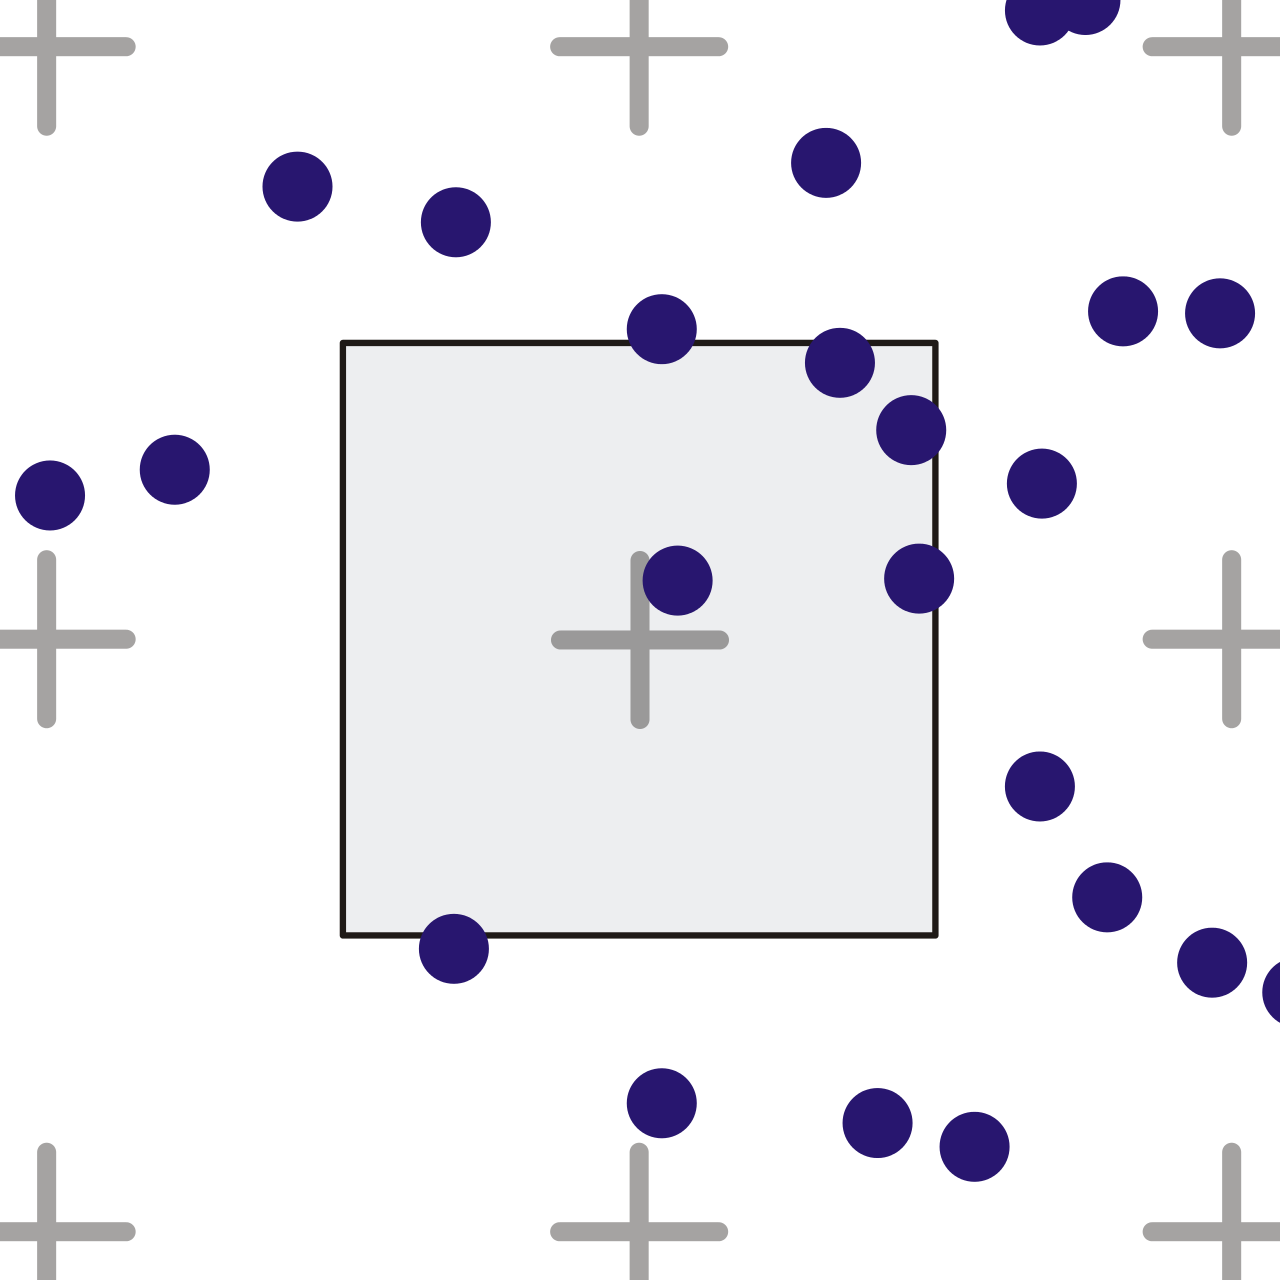
\includegraphics[scale=0.05]{./images/supersampling2.png}
\end{center}
\end{multicols}

\end{itemize}
\end{frame}


\section*{Другие алгоритмы.}
\begin{frame}[fragile]
\frametitle{Свёртка} 
\begin{center}
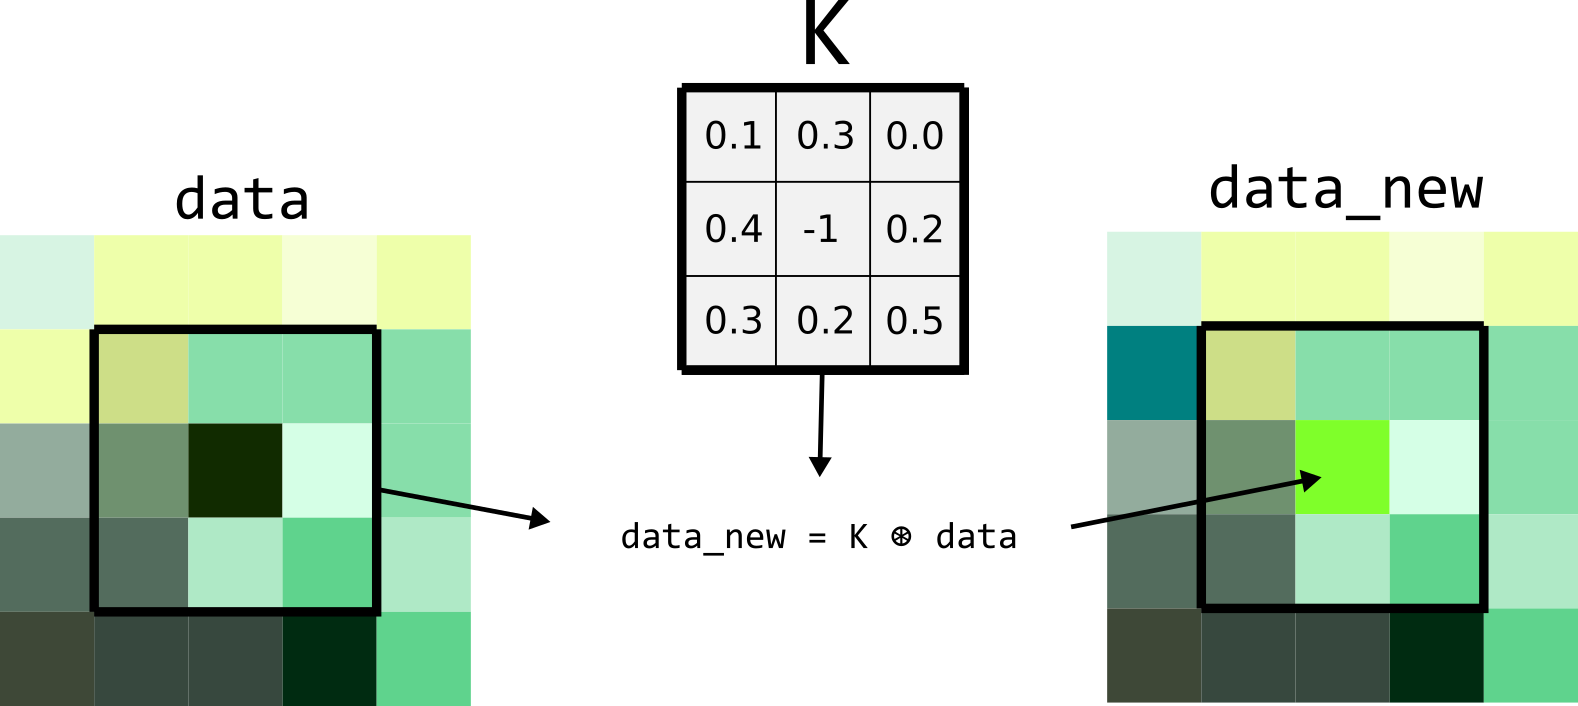
\includegraphics[scale=0.75]{./images/image_conv.png}
\end{center}
\end{frame}

\begin{frame}[fragile]
\frametitle{Трассировка лучей} 
\begin{center}
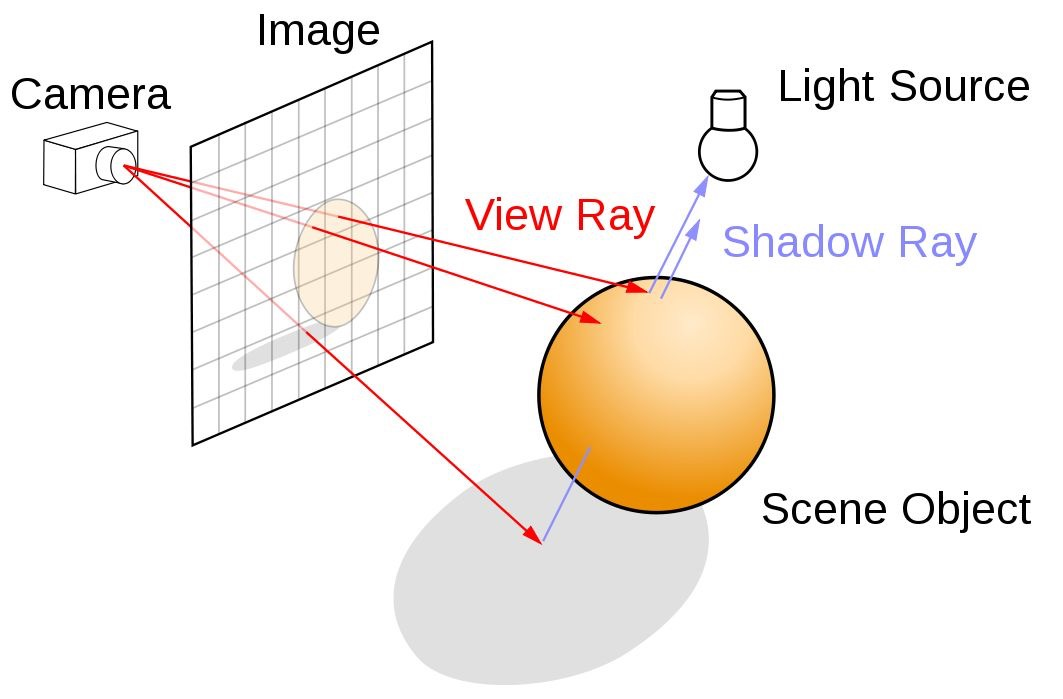
\includegraphics[scale=0.25]{./images/ray_tracing_image.jpg}
\end{center}
\end{frame}

\section*{Создание видео с помощью ffmpeg.}
\begin{frame}[fragile]
\frametitle{Создание видео с помощью ffmpeg} 
\begin{itemize}
\item Сначала создадим все кадры видео в виде jpeg картинок. Одна картинка на один кадр.
\item Потом используем консольныю программу \texttt{ffmpeg}:
\begin{lstlisting}
ffmpeg -framerate 30 -pattern_type glob -i '*.jpg'
       -c:v libx264 -pix_fmt yuv420p out.mp4
\end{lstlisting}
\end{itemize}
\end{frame}
\end{document}